\documentclass[12pt]{elsarticle}

% Add additional packages here if required
\usepackage{lineno, subfig}
\graphicspath{{imgs/}}
\modulolinenumbers[5]
\usepackage{float}
\usepackage{breqn}
\usepackage{xcolor}
\usepackage[utf8]{inputenc}
\usepackage[T1]{fontenc}
\usepackage{amsmath}
\usepackage{amsfonts}
\usepackage{amssymb}
\usepackage{mathtools}
\usepackage{graphicx}
% \usepackage{caption}
% \usepackage{subcaption}
\usepackage{booktabs}
\usepackage{optidef}
\usepackage{pstricks}
\usepackage{pst-all}
\usepackage{amsthm}
\usepackage{comment}
% \usepackage{pgfplots}

%\usepackage{soul}
\usepackage{mathrsfs}
\usepackage[ruled]{algorithm2e}
\usepackage{xspace}
%\usepackage{ulem}
\usepackage{multirow}

\usepackage{bigstrut}
\usepackage{url}
% \usepackage{algorithm}
\usepackage{algpseudocode}
\usepackage{enumerate}
\usepackage{makecell}
\newtheorem*{remark}{Remark}
\newtheorem{theorem}{Theorem}[section]
\newtheorem{corollary}{Corollary}[theorem]
\newtheorem{lemma}[theorem]{Lemma}
\allowdisplaybreaks

\usepackage[margin=1in]{geometry}
\bibliographystyle{elsarticle-num}
\newcommand{\LA}[1]{#1}
\newcommand{\CV}[1]{#1}
\newcommand{\LP}[1]{#1}
\definecolor{armygreen}{rgb}{0.19, 0.53, 0.43}
\newcommand{\JP}[1]{#1}

\newcommand{\VM}{{V^{}_{\mathcal M}}}
\newcommand{\VC}{{V^{}_{\mathcal C}}}

\newcommand{\EM}{{E^{}_{\mathcal M}}}
\newcommand{\EC}{{E^{}_{\mathcal C}}}

\newcommand{\TI}{{\mathcal{T}_i}}
\newcommand{\TB}{{\mathcal{T}_b}}

\newcommand{\Tm}{{\mathcal T_{\Delta_m}}}

\renewcommand\theadalign{bc}
\renewcommand\theadfont{\bfseries}
\renewcommand\theadgape{\Gape[4pt]}
\renewcommand\cellgape{\Gape[4pt]}
% \newcommand{\EMC}{{}}

% \usepackage{adjustbox}

\title{Drone Coverage Path Planning}


% Use the \authfn to add symbols for additional footnotes andi present addresses, if any. Usually start with 1 for notes about author contributions; then continuing with 2 etc if any author has a different present address.



\author[mymainaddress]{Lavinia Amorosi}
\ead{lavinia.amorosi@uniroma1.it}
\author[mymainaddress]{Paolo Dell'Olmo}
\ead{paolo.dellolmo@uniroma1.it}
\author[mysecondaryaddress]{Justo Puerto}
\ead{puerto@us.es}
\author[mysecondaryaddress]{Carlos Valverde \corref{mycorrespondingauthor}}
\ead{cvalverde@us.es}



\address[mymainaddress]{Department of Statistical Sciences, Sapienza University of Rome, Italy}
\address[mysecondaryaddress]{Department of Statistical Sciences and Operational Research, University of Seville, Spain}


\cortext[mycorrespondingauthor]{Corresponding author}



\begin{document}


\begin{frontmatter}


\begin{abstract}
We present a mixed-integer quadratic programming (MIQP) formulation for a drone coverage path planning problem. A single drone, with limited energy, must depart from a depot, cover a set of disjoint polygonal regions in the plane, and return to the depot to swap the battery and start a new tour, until all the regions are covered. Each region can be inspected at a discrete set of altitudes, each associated with a polygonal chain that defines the coverage pattern (altitude selection). A finite set of entry/exit points is associated with each region, allowing the drone to interrupt the coverage of a region and resume it later from a different point. The formulation embeds altitude selection, the geometry of the entry/exit points along the chain, and operation splitting under the endurance budget, using second-order-cone constraints for the Euclidean distances and a big-M linearization of the bilinear products between routing and distance/energy variables. We also propose an equivalent Edges-Approach reformulation that replaces vertex-visitation variables by edge-traversal variables and uses DFJ lazy subtour elimination, and a multi-phase constructive heuristic that produces feasible solutions in well under a second on all tested instances and is used to warm-start the exact solver. Two extensions are studied: splitting each coverage ring into $K\ge 1$ continuous arcs, so that entry and exit points need no longer coincide (with $K=1$ recovering the original model), and a wind-aware energy model in real joules with precomputable per-heading airspeed costs. On a testbed of 1080 artificial instances the Vertex-Approach formulation dominates without warm-start (94\% solved vs.\ 58\%), the two formulations agree within 1\% once warm-started, and the heuristic stays within 8\% of the exact mean objective at every scale; one split point per ring ($K=2$) already improves solutions by up to 25\%, with no further gains beyond $K=3$ on the tested instances.
\end{abstract}
\begin{keyword}
Drone coverage path planning, Mixed-Integer Quadratic Programming, UAV, Coverage patterns
\end{keyword}

\end{frontmatter}
\section{Introduction}
The optimization of unmanned aerial vehicle (UAV) operations is inherently multifaceted: it involves path planning, resource allocation, energy management, and collision avoidance in increasingly crowded airspaces. Determining the optimal route for a drone to cover a designated area while minimizing energy consumption and avoiding obstacles is a complex combinatorial and continuous optimization problem. When multiple drones are deployed simultaneously, coordination and scheduling add a further layer of difficulty, demanding algorithms that can handle dynamic environmental conditions and regulatory constraints.

Drones have been successfully adopted in many contexts, including disaster management~\cite{art:Chiaraviglio19,art:shi2024}, telecommunications for providing 5G coverage of rural zones~\cite{art:Amorosi19}, inspection of planar graphs~\cite{art:Amorosi2024,art:Amorosi2021,art:Amorosi2023}, 3D mapping and video surveillance~\cite{art:Nexand14}, and crop monitoring in agriculture~\cite{art:Tokekaretal16}. A broader survey of civil UAV applications is given in~\cite{art:Otto18}.

In this paper we focus on coverage of polygonal areas in the plane by a single drone. We propose a mixed-integer quadratic programming (MIQP) formulation that jointly optimizes the altitude, the entry and exit points, and the sequence of operations under a limited energy budget. Unlike existing two-stage approaches that first plan intra-region paths and then solve an inter-region routing problem, our formulation allows the drone to interrupt the coverage of a region and resume it later, potentially reducing total energy consumption. To tackle large instances, we also develop a multi-phase constructive heuristic that provides high-quality feasible solutions in well under a second and can be used to warm-start the exact solver. The main contributions of this paper are:
\begin{itemize}
    \item A MIQP formulation for the drone coverage path planning problem that integrates altitude selection, variable entry/exit points, and operation splitting under endurance constraints.
    \item An equivalent Edges-Approach reformulation that replaces vertex-visitation variables with edge-coverage variables and uses DFJ lazy subtour elimination, offering a different trade-off between constraint structure and relaxation strength.
    \item A multi-phase heuristic combining chain selection, region-level tour construction, greedy endurance-aware tour splitting, coordinate-descent entry-point optimization, and intra/inter-operation local search.
    \item A generalization to $K\ge 1$ split points per coverage ring, allowing entry and exit points to differ, with nested models ($K=1$ is the original formulation) and a knee in solution quality at $K=2$--$3$.
    \item A wind-aware energy extension in real joules with precomputable per-heading costs that preserves the MIQP structure and validates that optimal tours are robust to strong wind on the tested instances.
    \item A computational study on a testbed of 1080 artificial instances (540 per formulation) with varying numbers of regions, altitude levels, and endurance values, comparing the exact solver with and without warm-start against the standalone heuristic and the two equivalent MIQP formulations, plus split-point sweeps and wind-validation experiments.
\end{itemize}


\section{State of the art}
The coverage path planning problem (CPP) has been studied widely in the literature. A comprehensive survey that includes a taxonomy of CPP algorithms and drone-specific characteristics is presented in \cite{Sonawane2023}. Recent work can be grouped into three broad methodological streams.

\paragraph{Back-and-forth coverage patterns.}
Several authors adopt variants of the back-and-forth (also known as lawnmower or boustrophedon) strategy for intra-region coverage. \cite{Mu2023} propose an improved back-and-forth algorithm with a straight-turn mode to cover rectangular regions containing forbidden areas. \cite{Ahmed2024} develop a mathematical model and heuristic for energy-efficient multi-UAV multi-region CPP, using back-and-forth patterns with Bezier-curve smoothing to reduce energy consumption from turns; their optimization proceeds in two decoupled phases (intra-region path generation then inter-region routing). Similarly, \cite{Tripipicchio2023} generate waypoints for polygonal areas and apply smoothing to reduce flight time and memory footprint.

\paragraph{Two-stage and sequential approaches.}
Many methods first plan coverage paths within each region and then solve a separate routing problem. \cite{art:VAZQUEZ} present a CPP method for spraying drones that disinfect areas, tested on realistic scenarios. \cite{art:Wang2024} propose a two-stage method for mixed regions with limited energy: they shrink perimeters to generate optimal paths, then use dynamic programming to segment the overall path among multiple drones to satisfy energy limits. \cite{Li2025} develop a trajectory and velocity control approach for energy-efficient visual coverage of multiple terrestrial regions, solving the problem in four sequential stages.

\paragraph{Energy-aware formulations with altitude and speed control.}
The works most closely related to ours jointly consider energy, altitude, and speed decisions. \cite{Li2025} allow the UAV to change both velocity and altitude during its tour, optimizing visual coverage quality subject to energy constraints. Our approach differs from all of the above in that we allow the drone to interrupt coverage of a region and move to another one before returning, rather than fully covering each region in a single pass. This flexibility, enabled by the edge set $\mathcal E^{ext}$ in our model, can lead to shorter total tours compared to the two-stage paradigm, as illustrated in Section~\ref{section:description}.






\section{Problem Description}\label{section:description}
In this paper we study a drone coverage path planning problem. Given a set of non-overlapping polygonal areas to be visited, a single drone with limited endurance, and a depot, the problem consists of finding the set of tours (operations) starting and ending at the depot that the drone must perform in order to cover all areas. We assume that every region can be fully covered in a single operation, i.e.\ the drone has enough endurance to depart from the depot, cover a region, and return to the depot in one go.

Let $\mathcal R = \{1, \ldots, R\}$ be the set of regions to be covered, with $R=|\mathcal R|$. For each region $r\in\mathcal R$, the user specifies a set of polygonal chains $\mathcal T_r$, each at a different altitude and each defining a candidate coverage pattern. The visit of a region can be performed with interruptions: the drone may leave a region before completing its coverage and resume it from another point if doing so reduces the total energy consumption. The polygonal chain of a region can be traversed in both directions. For tractability, we assume that the number of interruptions per region is at most $R-1=|\mathcal R|-1$.

For each region $r\in\mathcal R$, we index the set of $2R$ candidate points along its selected chain by $\mathcal I_r=\{1,\ldots,2R\}$, partitioned into four subsets:
   \begin{itemize}
        \item $\mathcal I_S^r=\{1, 2\}$: the two endpoints at the start of the chain (each can act as a launching or retrieving point);
        \item $\mathcal I_L^r=\{3, 5,\ldots,2R-1\}$: the $R-1$ launching points;
        \item $\mathcal I_R^r=\{4, 6,\ldots, 2R\}$: the $R-1$ retrieving points;
        \item $\mathcal I_T^r=\{2R+1, 2R+2\}$: the two endpoints at the end of the chain (each can act as a launching or retrieving point).
   \end{itemize}
    The launch and retrieve points come in pairs: a launch point $2k+1$ is paired with the retrieve point $2k+2$ for $k=1,\dots,R-1$.

\begin{figure}[h!]
    \centering
    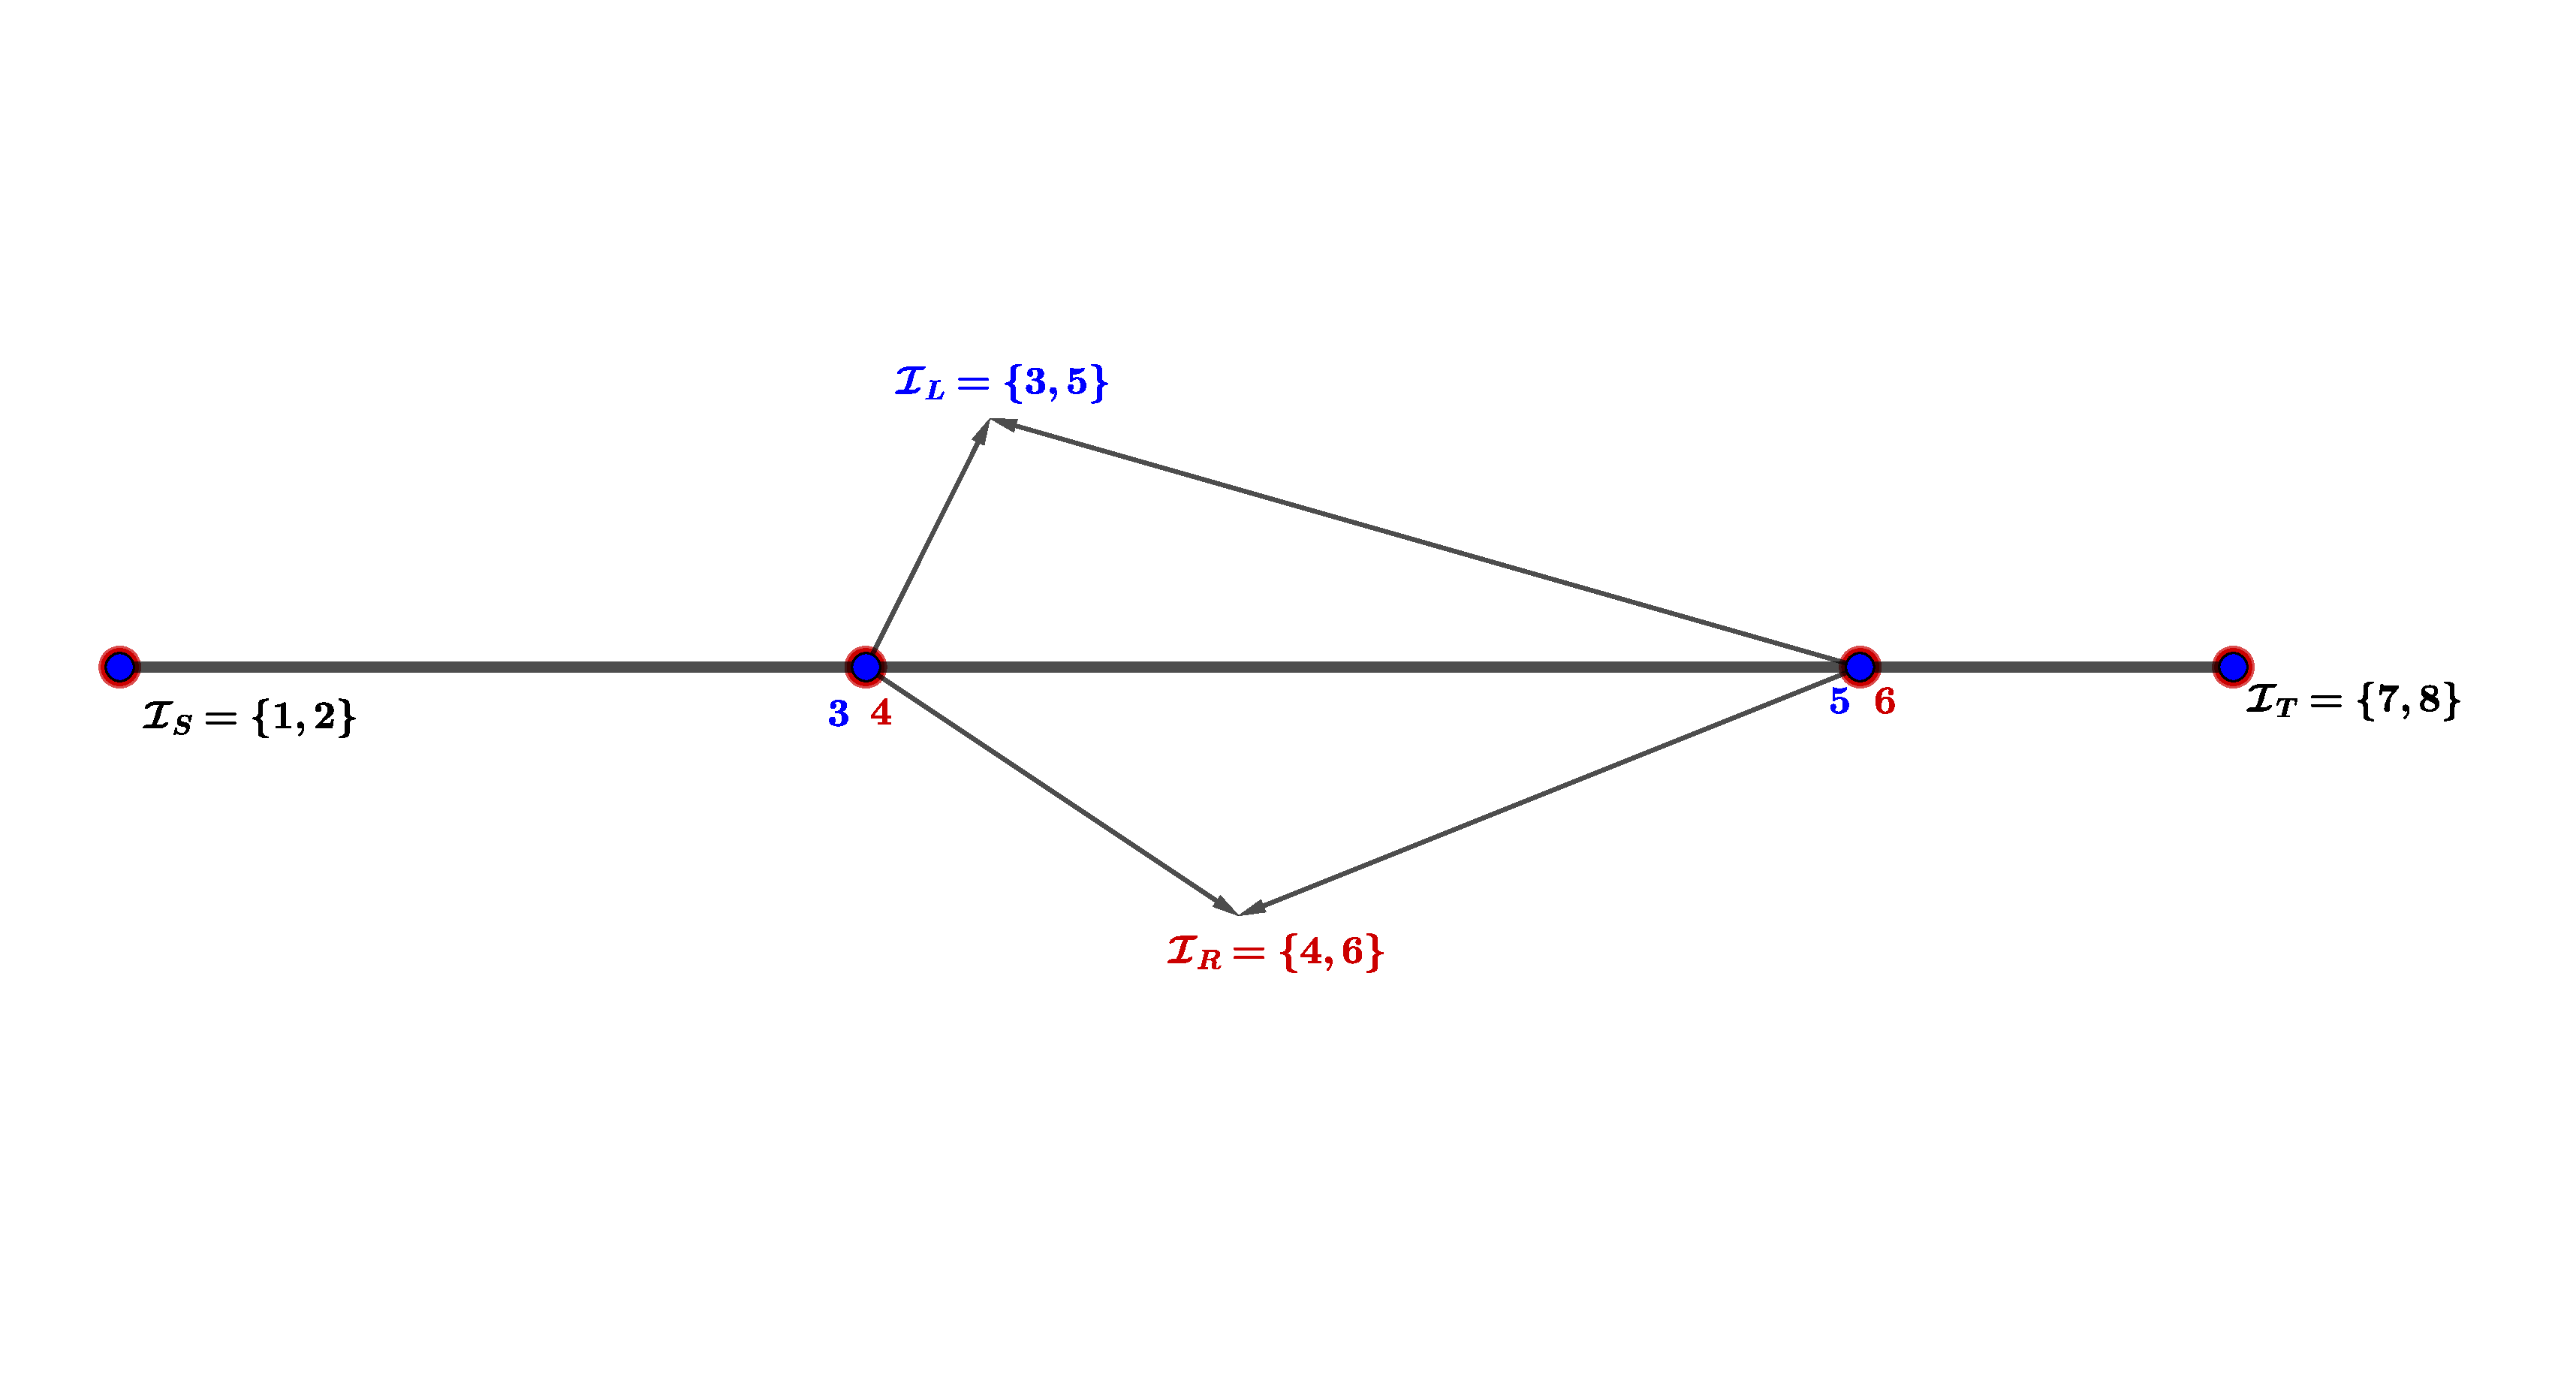
\includegraphics[width=0.8\linewidth]{pictures/set_I.pdf}
    \caption{Indexing of the candidate points along the chain of a single region ($R$ regions in total).}
    \label{fig:enter-label}
\end{figure}
We define the graph $\mathcal G=(\mathcal V=\{v_0\}\cup \mathcal V',\mathcal E=\mathcal E^{int}\cup\mathcal E^{ext})$, where:
\begin{itemize}
    \item $v_0=(0,0,0)$ denotes the depot.
    \item $\mathcal V'=\bigcup_{r\in\mathcal R}\{r\}\times\mathcal I_r$ is the set of all candidate points across regions. It is partitioned as $\mathcal V'=\mathcal V_S\cup\mathcal V_L\cup\mathcal V_R\cup\mathcal V_T$, where $\mathcal V_S=\bigcup_{r\in\mathcal R}\{r\}\times\mathcal I_S^r$, and similarly for $\mathcal V_L$, $\mathcal V_R$, $\mathcal V_T$.
    \item $\mathcal E^{int}=\{(v,v'):v=(r,i),v'=(r,i+1), \forall r\in\mathcal R, \forall i\in\mathcal I_r\setminus\{2R\}\}$ is the set of edges joining consecutive points on the same chain. It is partitioned into $\mathcal E_{LR}^{int}$ (forward edges) and $\mathcal E_{RL}^{int}$ (backward edges).
    \item $\mathcal E^{ext}=\{(v,v'):v=(r,i)\in \mathcal V'\setminus \mathcal V_R, v'=(r',i')\in \mathcal V'\setminus \mathcal V_L, r\neq r'\}$ is the set of arcs that join a non-retrieving point in one region to a non-launching point in another region.
    \item $\mathcal O$ is the set of operations, each a drone tour starting and ending at the depot $v_0$.
\end{itemize}

For each region $r\in\mathcal R$, the set $\mathcal T_r$ of polygonal chains contains the candidate coverage patterns for that region. Each chain $t\in\mathcal T_r$ is associated with an altitude $h_t$ and a sequence of segments $\{[Q^s,Q^{s+1}]:s\in\mathcal S_t\}$, where $Q^s,Q^{s+1}$ are the endpoints of segment $s$ and $\mathcal S_t=\{1,\ldots,S_t\}$ is the set of segments of the chain. The selection of one chain per region is a decision variable of the model.

We assume that air density, denoted by $\rho$, depends on height as given by the following function (derived from the ideal gas law and the International Standard Atmosphere model):
$$
\rho_h=\frac{p_0 M}{C_RT_0}\left(1-\frac{Lh}{T_0}\right)^{\frac{gM}{C_RL}-1},
$$
where the constants are:
\begin{itemize}
    \item $p_0=101325$ Pa: sea level standard atmospheric pressure;
    \item $T_0=288.15$ K: sea level standard temperature;
    \item $g=9.80665$ m/s$^2$: earth-surface gravitational acceleration;
    \item $L=0.0065$ K/m: temperature lapse rate;
    \item $C_R=8.31446$ J/(mol$\cdot$K): universal gas constant;
    \item $M=0.0289652$ kg/mol: molar mass of dry air.
\end{itemize}

We also assume that the wind has a constant direction represented by the unit vector $\vec{u}^w$. The magnitude of the wind speed depends on height following the power law of \cite{heier2014grid}:
$$
\nu^w_h=\nu^w_{10}\left(\frac{h}{10}\right)^a,
$$
where $\nu^w_{10}$ is the wind speed at 10\,m above ground and $a$ is the Hellmann exponent (which depends on the coastal location, terrain roughness, and air stability). The wind velocity vector at height $h$ is then $\vec{\nu}_h^w=\nu^w_h \vec{u}^w$.

Given the wind vector at altitude $h$, the drone airspeed required to maintain a ground velocity $\vec{\nu}$ is
$$
\vec{\nu}_h^d = \vec{\nu} - \vec{\nu}_h^w.
$$

\noindent Because the drone's position and the chosen chain are decision variables, the actual flight speed along an inter-region leg is unknown before the model is solved. To avoid bilinear terms, we approximate the direction of an inter-region leg $(r,r')$ by the unit vector from the centroid of $r$ to the centroid of $r'$, giving a precomputable ground speed $\vec\nu_{rr'h}^d$ (and hence energy) per region pair. The exact leg directions are recovered through the continuous position variables in the formulation.

One key feature of our problem setting is that the drone is not forced to fully explore one region before moving to another one. The edge set $\mathcal E^{ext}$ allows the drone to leave a region before completing its coverage and explore a different one. Other CPP contributions propose a two-stage approach, in which each region is fully covered first and then an inter-region routing problem is solved; this restriction can be suboptimal, as illustrated by the following example.

\paragraph{Illustrative example.}
Consider an instance with one large regular polygon of $n$ edges of length $l$ (a single region) and $n$ unit-size satellite regions placed externally at unit distance from each vertex of the polygon. Figure~\ref{fig:Exagon} shows the case $n=3$. Assume that the cost of covering the polygon is the same under both approaches. In our approach, the drone can leave the polygon at each vertex, cover the adjacent satellite, and resume the polygon. The satellite-covering cost is then $4n$ (unit inward detour, outward to satellite, back, unit back to polygon). In the two-stage approach, the satellite regions must be covered by separate trips from the depot; the best inter-region travel has cost at least $(n-1)l$, where $l$ is the polygon edge length. The ratio of the two cost gaps is then $(n-1)l/(4n)$, which grows with $l$. The worst case for the two-stage gap among regular polygons is the triangle ($n=3$), giving a ratio of $l/6$.

\begin{figure}
    \centering
    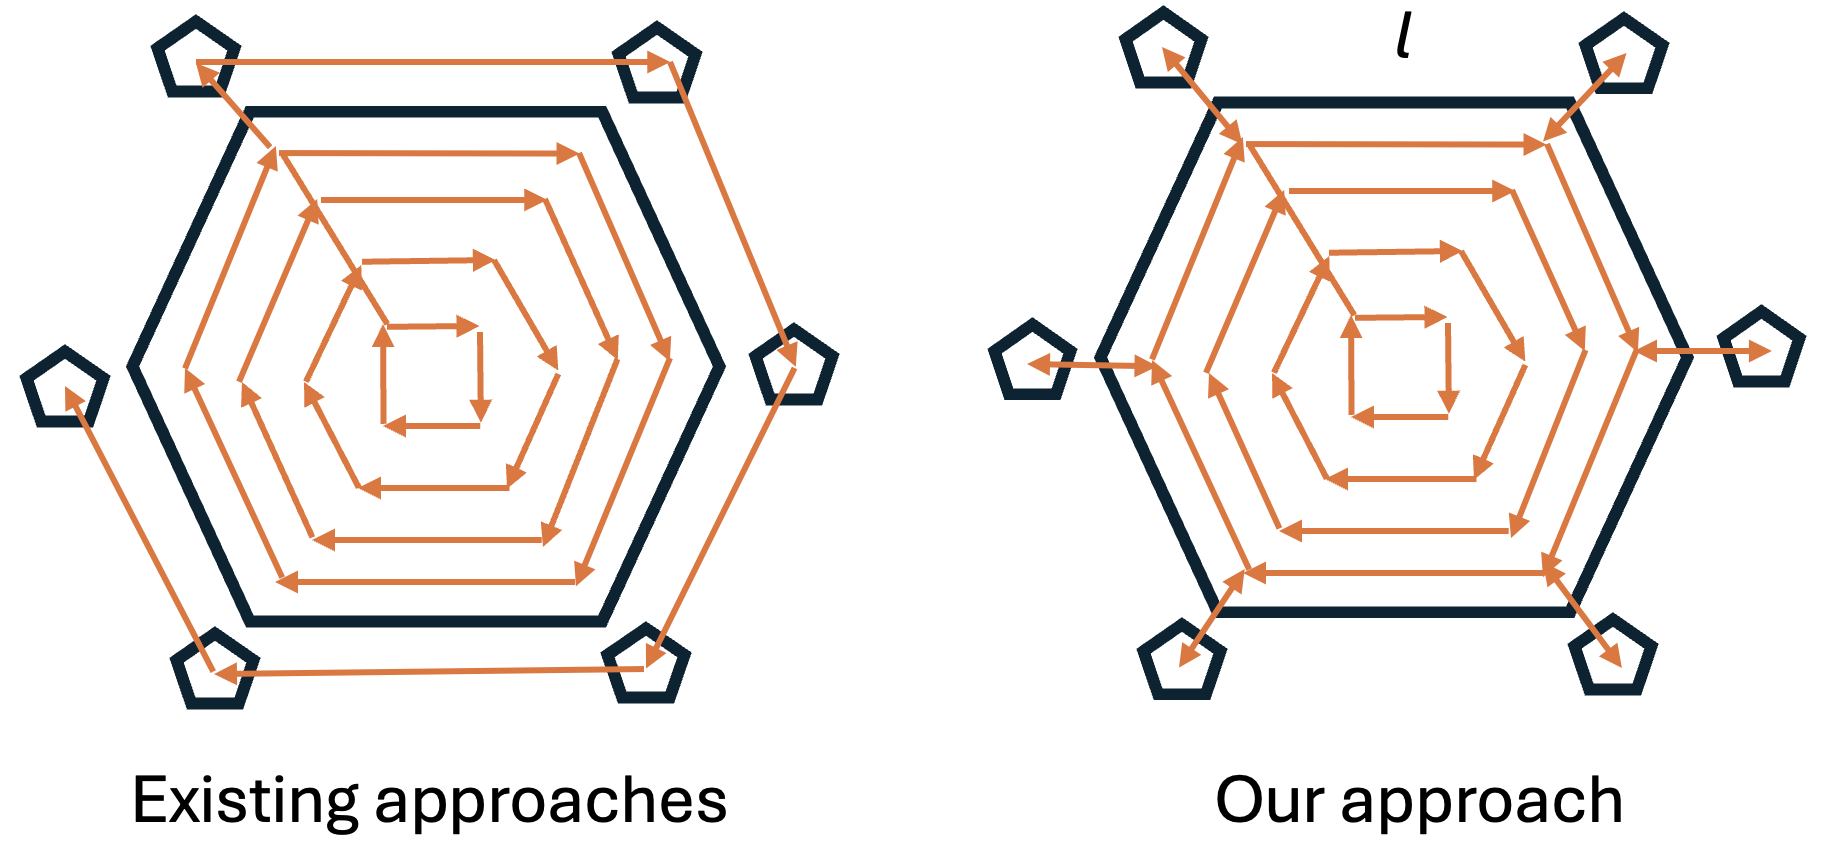
\includegraphics[width=0.8\linewidth]{pictures/Exagon.png}
    \caption{Comparison of the proposed approach (left) and the two-stage approach (right) for a triangle with three satellite regions.}
    \label{fig:Exagon}
\end{figure}

It should be noted that our approach does not \emph{force} the drone to leave a region before completing it; it merely \emph{allows} this whenever doing so reduces the total cost.

\paragraph{Complexity.} The problem is NP-hard: even with fixed chains, fixed entry/exit positions, and a single altitude, sequencing the inter-region legs under the endurance budget contains the travelling salesman problem (one region per operation with unit endurance) and the capacitated vehicle routing problem (packing multiple regions per operation) as special cases.  This justifies both the exact MIQP approach for small instances and the heuristic of Section~\ref{sec:heuristic} for larger ones.

\section{Mathematical Formulation}\label{sec:formulation}
This section presents a mixed-integer quadratic programming formulation for the problem outlined in Section~\ref{section:description}. The model has four families of constraints: \emph{(i)} location constraints, which determine the placement of the entry/exit points along the polygonal chain of each region; \emph{(ii)} drone path constraints, which govern the sequence of operations and eliminate subtours; \emph{(iii)} distance constraints, which model the movements between points; and \emph{(iv)} consumption constraints, which translate distances into energy and enforce the endurance budget. The decision variables used in the formulation are summarized in Tables~\ref{table:variables1} and~\ref{table:variables2}.

\begin{table}[t]
\centering
\caption{Main notation. Decision variables are detailed in Tables~\ref{table:variables1}--\ref{table:variables2}; constraint families Loc-C, Path-C, Dist-C, Ener-C, Dep-C, End-C, VI-C, S-C and W-C are defined in Sections~\ref{sec:formulation}--\ref{sec:windaware}.}
\label{tab:notation}
\begin{tabular}{ll}
\toprule
Symbol & Meaning \\
\midrule
\multicolumn{2}{l}{\textit{Sets and indices}} \\
$\mathcal R$, $R=|\mathcal R|$ & regions and their number; $r,r'$ index regions \\
$\mathcal T_r$, $\mathcal S_t$ & candidate chains of $r$ ($t$ index) and segments of $t$ ($s$ index) \\
$\mathcal I_r$ & candidate entry/exit points of $r$ ($2R$ per region) \\
$\mathcal G=(\mathcal V,\mathcal E)$ & flight graph; $v_0$ depot, $\mathcal V'$ region vertices \\
$\mathcal E^{int}$, $\mathcal E^{ext}$ & intra-region (chain) edges and inter-region legs \\
$\mathcal O$ & operations (depot tours); $o$ index \\
\multicolumn{2}{l}{\textit{Parameters}} \\
$h_t$, $\rho_h$, $\vec\nu_h^w$ & chain altitude, air density, wind velocity at height $h$ \\
$L(s)$, $Q^s$ & length and endpoints of chain segment $s$ \\
$W^{\max}$ & endurance (energy) budget per operation \\
\multicolumn{2}{l}{\textit{Key decision variables}} \\
$\alpha_t$ & 1 if chain $t$ is selected \\
$x_{vv'}^o$, $y_v^o$, $\zeta^o$ & traversal, visitation and idle-operation indicators \\
$\lambda_v$, $\gamma_v$, $\mu_v^{ts}$ & chain position, in-segment offset, segment assignment \\
$d_{uv}$, $w_{uv}$, $\ell_{uv}^o$ & distance, energy and per-operation linearized cost \\
\bottomrule
\end{tabular}
\end{table}


Table~\ref{tab:notation} collects the notation used throughout the model. Constraint families are labelled by block: Loc-C (location), Path-C (routing), Dist-C (distances), Ener-C (energy), Dep-C (depot legs), End-C (endurance), VI-C (valid inequalities), S-C (split points) and W-C (wind-aware energy); primed variants (e.g.\ Path-C$'_4$) denote the Edges-Approach counterparts introduced in Section~\ref{sec:alternative}.



\begin{table}[h!]
\centering
\caption{Corrected Table of Variables}
\label{table:variables1}
\resizebox{\textwidth}{!}{%
\begin{tabular}{llll}
\toprule
\textbf{Name} & \textbf{Domain} & \textbf{Range} & \textbf{Description} \\
\midrule
$\mu_{v}^s$ & $\mathcal V_2 \times \{s\in\mathcal S_t:t\in\mathcal T_r\}$ & $\{0,1\}$ & 1, if vertex $v=(r,i)$ is located at the segment $s\in \mathcal S_t$, where $t\in\mathcal T_r$. \\
$\alpha_{t}$ & $\{t\in\mathcal T_r:r\in\mathcal R\}$ & $\{0, 1\}$ & 1, if polygonal chain $t$ is selected. \\
$x_{vv'}^o$ & $\mathcal E \times \mathcal O$ & $\{0, 1\}$ & 1, if the drone goes from vertex $v$ to vertex $v'$ in operation $o$. \\
$y_{v}^o$ & $\mathcal V' \times \mathcal O$ & $\{0, 1\}$ & 1, if vertex $v$ is visited during operation $o$. \\
$\zeta^o$ & $\mathcal O$ & $\{0, 1\}$ & 1, if all vertices are visited before starting operation $o$. \\
$k^o$ & $\mathcal O$ & $[1, 2,\ldots, |\mathcal V'|]$ & number of vertices visited in operation $o$. \\
$\varphi_{rr'}$ & $\{(r,r')\in\mathcal R \times \mathcal R:r\neq r'\}$ & $\{0, 1\}$ & 1, if the drone moves from region $r$ to region $r'$ at the height selected to visit region $r$. \\
$\psi_{rr'}$ & $\{(r,r')\in\mathcal R \times \mathcal R:r\neq r'\}$ & $\{0, 1\}$ & 1, if the height selected to visit region $r$ is lower than the height selected to visit region $r'$. \\
\bottomrule
\end{tabular}%
}
\end{table}
\begin{table}[h!]
\centering
\caption{Continuous variables}
\label{table:variables2}
\resizebox{\textwidth}{!}{%
\begin{tabular}{llll}
\toprule
\textbf{Name} & \textbf{Domain} & \textbf{Range} & \textbf{Description} \\
\midrule
$P_v$ & $\mathcal V'$ & $\mathbb{R}^3$ & Coordinates of the point associated to vertex $v$. \\
$\gamma_v$ & $\mathcal V'$ & $[0,1]$ & Position of vertex $v$ within its selected segment. \\
$\lambda_v$ & $\mathcal V'$ & $[0, S_t]:t\in\mathcal T_r$ & Global parametrization of vertex $v$ on the selected chain. \\
$\eta_v^{ts}$ & $\mathcal V' \times \{(t,s):t\in\mathcal T_r,s\in\mathcal S_t\}$ & $[0,1]$ & Linearization of $\gamma_v\cdot\mu_v^{ts}$. \\
$dfs_v$ & $\mathcal V'$ & $[0, L_{\max}]$ & Cumulative distance from the start of the chain to vertex $v$. \\
$efs_v$ & $\mathcal V'$ & $[0, W_{\max}]$ & Cumulative energy from the start of the chain to vertex $v$. \\
$d_{vv'}$ & $\mathcal E$ & $\mathbb{R}^+$ & Distance between vertex $v$ and vertex $v'$. \\
$d_{vv'}^{xy}$ & $\mathcal E^{ext}$ & $\mathbb{R}^+$ & Horizontal distance between $v$ and $v'$. \\
$d_{vv'}^{z}$ & $\mathcal E^{ext}$ & $\mathbb{R}^+$ & Vertical distance between $v$ and $v'$. \\
$w_{vv'}$ & $\mathcal E$ & $\mathbb{R}^+$ & Energy consumption between $v$ and $v'$. \\
$u_v^o$ & $\mathcal V' \times \mathcal O$ & $[1, |\mathcal V'|]$ & Position of $v$ in the tour of operation $o$ (MTZ). \\
$\ell_{uv}^o$ & $\mathcal E \times \mathcal O$ & $[0, \infty)$ & Linearization of $x_{uv}^o\cdot d_{uv}$ (objective) and $x_{uv}^o\cdot w_{uv}$ (endurance). \\
$\rho_r$ & $\mathcal R$ & $[0,\rho(0)]$ & Air density at the height selected for region $r$. \\
\bottomrule
\end{tabular}}
\end{table}


\subsection{Location constraints}

The entry and exit vertices are not fixed waypoints. Each vertex $v=(r,i)$ floats along the coverage chains of its region, so the model must decide two things for every vertex: (a) \emph{which} chain (altitude) it lies on and (b) \emph{where} on that chain it sits. We encode (a) with a one-hot chain selector $\alpha_t$ and a segment assignment $\mu_v^{ts}$, and (b) with a continuous in-segment offset $\gamma_v\in[0,1]$; a single curvilinear coordinate $\lambda_v$ then orders all vertices along the chain (Fig.~\ref{fig:parameterization}). The constraints below build this positioning in three steps: coordinates from assignment (Loc-C$_1$), one chain per region (Loc-C$_2$--C$_3$), and the $\lambda$ ordering with endpoint fixing (Loc-C$_4$--C$_8$).

For each vertex $v=(r,i)\in\mathcal V'$ we define its spatial coordinates $P_v=(P_v^x,P_v^y,P_v^z)\in\mathbb R^3$. Let $\mu_v^{ts}$ be a binary variable that is one if vertex $v$ is placed on segment $s$ of chain $t$, and let $\gamma_v\in[0,1]$ denote the relative position within that segment. The product $\gamma_v\cdot\mu_v^{ts}$ is linearized via the auxiliary continuous variable $\eta_v^{ts}$, constrained by standard Fortet inequalities ($0\le\eta_v^{ts}\le\mu_v^{ts}$, $\gamma_v-(1-\mu_v^{ts})\le\eta_v^{ts}\le\gamma_v$). The coordinates of $v$ are then given by:

\begin{align}
    P_v &= \sum_{t\in\mathcal T_r}\sum_{s\in\mathcal S_t}
          \bigl[ \mu_v^{ts} Q^s + \eta_v^{ts} (Q^{s+1}-Q^s) \bigr],
          && \forall v=(r,i)\in\mathcal V', \label{eq:location_1}\tag{Loc-C$_1$}\\[2mm]
    P_v^z &= \sum_{t\in\mathcal T_r}\sum_{s\in\mathcal S_t}
            \mu_v^{ts}\,h_t,
          && \forall v=(r,i)\in\mathcal V', \label{eq:location_1z}\tag{Loc-C$_1^z$}
\end{align}

\noindent where $h_t$ is the altitude of chain $t$. Constraint~\eqref{eq:location_1z} defines the vertical coordinate independently, since each chain $t$ is associated with a single flight altitude. The segment assignment and chain selection are enforced by:

\begin{align}
    \sum_{s\in\mathcal S_t} \mu_v^{ts} &= \alpha_t,
          && \forall v=(r,i)\in\mathcal V',\; \forall t\in\mathcal T_r,
          \label{eq:location_2}\tag{Loc-C$_2$}\\
    \sum_{t\in\mathcal T_r} \alpha_t &= 1,
          && \forall r\in\mathcal R,
          \label{eq:location_3}\tag{Loc-C$_3$}
\end{align}

\noindent where $\alpha_t$ is a binary variable that is one if chain $t$ is selected. The parametrization of vertices along the chain is defined via the continuous variable $\lambda_v\in[0,S_t]$:

\begin{align}
    \lambda_v &= \sum_{t\in\mathcal T_r}\sum_{s\in\mathcal S_t}
                (s-1)\mu_v^{ts} + \gamma_v,
          && \forall v\in\mathcal V',
          \label{eq:location_4}\tag{Loc-C$_4$}\\
    \lambda_v &= 0,
          && \forall v=(r,1),(r,2),
          \label{eq:location_5}\tag{Loc-C$_5$}
\end{align}

\noindent with the following fixing at the chain endpoints (start vertices $(r,1),(r,2)$ and end vertices $(r,2R+1),(r,2R+2)$):

\begin{align}
    \mu_v^{t0} &= \alpha_t,
          && \forall v=(r,1),(r,2),\; \forall t\in\mathcal T_r,
          \label{eq:location_5b}\tag{Loc-C$_{5b}$}\\
    \lambda_u &\le \lambda_v,
          && \forall (u,v)\in\mathcal E_{RL}^{int}\cup\mathcal E_{RL}^{S}\cup\mathcal E_{RL}^{T},
          \label{eq:location_6}\tag{Loc-C$_6$}\\
    \lambda_u &= \lambda_v,
          && \forall (u,v)\in\mathcal E_{LR}^{int}\cup\mathcal E_{LR}^{S}\cup\mathcal E_{LR}^{T},
          \label{eq:location_7}\tag{Loc-C$_7$}\\
    \lambda_v &= \sum_{t\in\mathcal T_r} S_t\,\alpha_t,
          && \forall v=(r,2R+1),(r,2R+2),
          \label{eq:location_8}\tag{Loc-C$_8$}\\
    \mu_v^{t,S_t-1} &= \alpha_t,
          && \forall v=(r,2R+1),(r,2R+2),\; \forall t\in\mathcal T_r.
          \label{eq:location_8b}\tag{Loc-C$_{8b}$}
\end{align}

Constraint~\eqref{eq:location_4} defines $\lambda_v$ as the cumulative length from the chain start to the point, expressed as the index of the selected segment (minus one) plus the offset $\gamma_v$ within that segment. Constraint~\eqref{eq:location_5} fixes the parametrization at zero for the start vertices. Constraint~\eqref{eq:location_5b} fixes the first segment for start vertices. Constraints~\eqref{eq:location_6} and~\eqref{eq:location_7} enforce the traversal order and the coincidence of launch--retrieve pairs, respectively. Constraint~\eqref{eq:location_8} sets $\lambda$ to the total chain length for the end vertices, and~\eqref{eq:location_8b} fixes the last segment for those vertices. Together, Loc-C$_1$--C$_8$ pin every vertex to exactly one point of exactly one chain; the routing layer that follows can therefore treat the positions $P_v$ as variables fully determined by the assignment decisions.

\begin{figure}
    \centering
    \includegraphics[width=0.8\linewidth]{to_find_ourselves.png}
    \caption{Parameterization of vertices}
    \label{fig:parameterization}
\end{figure}

\subsection{Drone path constraints}
With vertex positions established, the next block strings vertices into depot tours. Each operation $o$ is a closed walk starting and ending at $v_0$ that visits a subset of vertices, every vertex is visited exactly once across all operations, and no tour contains a cycle detached from the depot. We model this with traversal variables $x_{vv'}^o$ (which legs are flown in which operation) and visitation variables $y_v^o$ derived from them; flow conservation (Path-C$_2$) plus depot departure/arrival (Path-C$_1$, Path-C$_3$) shape each operation, while Miller--Tucker--Zemlin ordering variables $u_v^o$ (Path-C$_7$) rule out subtours. Operations are allowed to be idle once everything is covered, via the flag $\zeta^o$. The variables modeling the path are as follows. Let $x_{vv'}^o$ be a binary variable that is one if the drone goes from vertex $v$ to vertex $v'$ in operation $o$. Let $y_v^o$ be a binary variable that is one if the vertex $v$ is visited during the operation $o$. Let also $\zeta^o$ be a binary variable that is one if all vertices are visited before starting the operation $o$. We count the number of vertices visited in operation $o$ by means of the integer variable $k^o$. Additionally, $u_v^o$ is a continuous variable that represents the position of vertex $v$ in the tour of operation $o$, used in the subtour elimination constraints.

\begin{align*}
\sum_{v'\in \mathcal V} x_{v_0v'}^{o}&=1-\zeta^o,&\quad \forall o\in\mathcal O,\label{eq:drone_path_1}\tag{Path-C$_1$}\\
\sum_{v'\in\mathcal V} x_{v'v}^{o}-\sum_{v'\in\mathcal V}x_{vv'}^{o}&=0,&\quad\forall v\in\mathcal V',\forall o\in\mathcal O,\label{eq:drone_path_2}\tag{Path-C$_2$}\\
\sum_{v'\in\mathcal V} x_{v'v_0}^{o}&=1-\zeta^o,&\quad\forall o\in\mathcal O,\label{eq:drone_path_3}\tag{Path-C$_3$}\\
\sum_{v'\in\mathcal V} x_{vv'}^o&=y_{v}^o,&\quad\forall v\in\mathcal V,\forall o\in\mathcal O,\label{eq:drone_path_4}\tag{Path-C$_4$}\\
\sum_{v'\in\mathcal V} x_{v'v}^o&=y_{v}^o,&\quad\forall v\in\mathcal V,\forall o\in\mathcal O,\label{eq:drone_path_5}\tag{Path-C$_5$}\\
\sum_{o\in\mathcal O}y_v^o&=1,&\quad\forall v\in\mathcal V',\label{eq:drone_path_6}\tag{Path-C$_6$}\\
u_v^o - u_{v'}^o + 1 &\leq |\mathcal V'|(1 - x_{vv'}^o), &\quad\forall v,v'\in\mathcal V':v\neq v',\forall o\in\mathcal O,\label{eq:drone_path_7}\tag{Path-C$_7$}\\
1 \leq u_v^o &\leq |\mathcal V'|, &\quad\forall v\in\mathcal V',\forall o\in\mathcal O.\label{eq:drone_path_7b}\tag{Path-C$_{7b}$}\\
\sum_{o\in\mathcal O} x_{vv'}^o &= 1, &\forall v,v'\in\mathcal V':(v,v')\in\mathcal E_{RL}^{int}\cup\mathcal E_{RL}^{S}\cup\mathcal E_{RL}^{T}\label{eq:drone_path_8}\tag{Path-C$_8$}.
\end{align*}
Constraints \eqref{eq:drone_path_1} ensure that the drone exits from the depot if there is a vertex that is not already visited in operation $o$. Constraints \eqref{eq:drone_path_2} are the flow conservation constraints. Constraints \eqref{eq:drone_path_3} guarantee that drone operation ends in the depot if there is a vertex that has not been visited in operation $o$. Constraints \eqref{eq:drone_path_4} and \eqref{eq:drone_path_5} ensure that the vertex $v$ is visited if there is a path passing through this vertex. Constraints \eqref{eq:drone_path_6} impose that every vertex must be visited in some operation. Inequalities \eqref{eq:drone_path_7} are the Miller--Tucker--Zemlin (MTZ) subtour elimination constraints~\cite{MTZ1960}, which use the auxiliary variables $u_v^o$ to enforce that the tours in each operation contain no cycles that exclude the depot. The bounds \eqref{eq:drone_path_7b} define the range of these continuous variables. Finally, constraints \eqref{eq:drone_path_8}
guarantee that each polygonal chain is completely traversed by requiring that all edges of the path graph associated with each region are traversed in some operation.

\subsubsection*{Valid Inequalities}
The path constraints above admit many symmetric solutions (e.g.\ permuting idle operations) that slow down branch-and-bound without changing the optimum. To tighten the relaxation, the inequalities VI-C$_1$--C$_4$ cut off such fractional and symmetric solutions: they force idle operations to come last, count how many vertices each operation covers, and tie that count to the idle flag so the relaxation ``sees'' that an active operation must do useful work. Concretely, let $\zeta^o$ be a binary variable that takes the value of one if all vertices have been visited before starting the operation $o$, and zero otherwise. If this is the case, then all vertices must also be visited before the operation $o+1$. Therefore, the $\zeta$ variables must satisfy the following monotonicity constraint:

\begin{equation}\label{eq:mon}\tag{VI-C$_1$}
\zeta^o\leq \zeta^{o+1},\quad\forall o\in\mathcal O\setminus\{O\}.
\end{equation}

We define $k^o$ as the number of vertices visited during the operation $o$, excluding the depot. The variables $y$ can be used to determine this quantity, where we recall that $y_v^{o}$ equals one if the vertex $v$ is visited in operation $o$. Thus:

\begin{equation}\label{eq:k}\tag{VI-C$_2$}
k^o=\sum_{v\in\mathcal V'} y_{v}^o, \quad\forall o\in\mathcal O.
\end{equation}

If $\zeta^o$ is equal to one, it implies that all vertices in $\mathcal V'$ must have been visited in previous operations. This relationship is enforced through the following inequality:

\begin{equation}\label{eq:VI-1}\tag{VI-C$_3$}
\sum_{o'=1}^{o-1} k^{o'}\geq |\mathcal V'| \zeta^o,\quad\forall o\in\mathcal O.
\end{equation}

To refine the feasible solution space, we assume, without loss of generality, that an operation $o$ cannot consists in remaining at the depot, if there are still targets left to visit. This requirement is ensured by the following constraint:

\begin{equation}\label{eq:VI-2}\tag{VI-C$_4$}
k^o\geq 1-\zeta^o,\quad\forall o\in\mathcal O.
\end{equation}


\subsection{Distance constraints}

Routing needs leg lengths, but vertex positions are variables, so distances cannot be precomputed---except along a chain, where the $\lambda$ ordering makes them trivial. The construction is therefore twofold: on intra-region edges the length is read off an accumulated-distance variable $dfs_v$ (a difference of two such variables, Dist-C$_1$--C$_2$), and on inter-region legs explicit distance variables are bounded below by the Euclidean norm via a second-order cone (Dist-C$_3$--C$_6$). Since the objective minimizes total length, each ``$\ge$'' bound is tight at optimality. We consider first pairs of vertices belonging to the same region, then pairs in different regions.

\paragraph{Intra-region distances.}
For each region $r$, the polygonal chain $t$ is composed of segments $\mathcal S_t$ of known lengths $L(s)=\|Q^{s+1}-Q^s\|_2$. Rather than introducing bilinear products $\mu_v^s\mu_{v'}^{s'}$, we define an auxiliary continuous variable $dfs_v$ that accumulates the distance from the start of the chain to vertex $v$:

\begin{align}
    dfs_v &= \sum_{t\in\mathcal T_r}\sum_{s\in\mathcal S_t}
            \bigl[ \operatorname{cum\_before}(s)\,\mu_v^{ts}
            + L(s)\,\eta_v^{ts} \bigr],
            && \forall v\in\mathcal V',
            \label{eq:dfs}\tag{Dist-C$_1$}\\[2mm]
    d_{uv} &= dfs_v - dfs_u,
            && \forall (u,v)\in\mathcal E_{RL}^{int},
            \label{eq:dist_int_rl}\tag{Dist-C$_2$}\\
    d_{uv} &= 0,
            && \forall (u,v)\in\mathcal E_{LR}^{int},
            \label{eq:dist_int_lr}\tag{Dist-C$_3$}
\end{align}

\noindent where $\operatorname{cum\_before}(s)=\sum_{s'<s}L(s')$ is the length of the chain up to the start of segment $s$, and $\eta_v^{ts}=\gamma_v\cdot\mu_v^{ts}$ is the same linearization variable used in~\eqref{eq:location_1}. For RL edges the distance is simply the difference of cumulative distances from the chain start; for LR edges the two vertices coincide ($\lambda_u=\lambda_v$ from~\eqref{eq:location_7}) so the distance is zero.

\paragraph{Inter-region distances.}
For vertices in different regions we decompose the movement into horizontal and vertical components. Let $d_{vv'}^{xy}$ and $d_{vv'}^z$ be continuous variables representing the horizontal and vertical distances, respectively. The total distance is then:

\begin{align}
    d_{vv'} &= d_{vv'}^{xy} + d_{vv'}^z,
            && \forall (v,v')\in\mathcal E^{ext},
            \label{eq:dist_ext_sum}\tag{Dist-C$_4$}\\
    d_{vv'}^{xy} &\ge \bigl\| (P_v^x,P_v^y) - (P_{v'}^x,P_{v'}^y) \bigr\|_2,
            && \forall (v,v')\in\mathcal E^{ext},
            \label{eq:dist_ext_xy}\tag{Dist-C$_5$}\\
    d_{vv'}^z &\ge P_v^z - P_{v'}^z,
            && \forall (v,v')\in\mathcal E^{ext},
            \label{eq:dist_ext_z1}\tag{Dist-C$_6$}\\
    d_{vv'}^z &\ge P_{v'}^z - P_v^z,
            && \forall (v,v')\in\mathcal E^{ext}.
            \label{eq:dist_ext_z2}\tag{Dist-C$_7$}
\end{align}

Constraint~\eqref{eq:dist_ext_xy} is a second-order cone constraint that computes the Euclidean horizontal distance. Constraints~\eqref{eq:dist_ext_z1}--\eqref{eq:dist_ext_z2} give the absolute vertical difference via a standard linearization. At this point every edge $(u,v)\in\mathcal E$ carries a well-defined length $d_{uv}$: exact along chains, Euclidean across regions. The next block converts these lengths into energy.


\subsection{Consumption constraints}

The energy consumed by the drone is modeled using the drag formula $w = \tfrac12 A c\,\rho\,\nu\,d$, where $A$ is the frontal area, $c$ the drag coefficient, $\rho$ the air density, $\nu$ the drone speed, and $d$ the travelled distance. We define the constants $E^{xy}=E^{z}=\tfrac12 cA$ for brevity. \emph{Units:} throughout Sections~\ref{sec:formulation}--\ref{sec:splitpoints} energy is measured in the model's nominal units (drag constants at cruise speed, calm air), which we write as pseudo-joules (pseudo-J) to distinguish them from the real joules of the wind-aware extension in Section~\ref{sec:windaware}. As with distances, we treat intra-region and inter-region pairs separately.

\paragraph{Intra-region energy.}
Following the same approach as for distances, we introduce an auxiliary continuous variable $efs_v$ that accumulates the energy from the start of the chain to vertex $v$:

\begin{align}
    efs_v &= \sum_{t\in\mathcal T_r}\sum_{s\in\mathcal S_t}
            C_{ts}\bigl[ \operatorname{cum\_before}(s)\,\mu_v^{ts}
            + L(s)\,\eta_v^{ts} \bigr],
            && \forall v\in\mathcal V',
            \label{eq:efs}\tag{Ener-C$_1$}\\[2mm]
    w_{uv} &= efs_v - efs_u,
            && \forall (u,v)\in\mathcal E_{RL}^{int},
            \label{eq:ener_int_rl}\tag{Ener-C$_2$}\\
    w_{uv} &= 0,
            && \forall (u,v)\in\mathcal E_{LR}^{int},
            \label{eq:ener_int_lr}\tag{Ener-C$_3$}
\end{align}

\noindent where $C_{ts}=E^{xy}\rho_t\,\nu_{ts}^d$ is the energy per unit distance on segment $s$ of chain $t$, computed as a constant during pre-processing. The drone ground speed $\nu_{ts}^d$ along segment $s$ is obtained from $\vec\nu_{ts}^d = v_{\text{cruise}}\frac{Q^{s+1}-Q^s}{\|Q^{s+1}-Q^s\|} - \vec\nu_{h}^w$ for forward traversal (and the opposite sign for backward traversal).

\paragraph{Inter-region energy.}
Flying from region $r$ to region $r'$ burns horizontal energy at the air density of the departure altitude and vertical energy only for the climbed part. Both depend on decisions: the departure chain (via $\alpha_t$) selects the density, and the relative heights of $r$ and $r'$ decide the climb direction. To disentangle the two effects we introduce auxiliary binaries: $\varphi_{rr'}$ is one if the drone departs from region $r$ at the altitude selected for that region, and $\psi_{rr'}$ is one if the altitude of $r$ is lower than that of $r'$. Each branch of~\eqref{eq:ener_ext} below is then a product of binaries with distances, linearized exactly with Fortet envelopes. The energy consumption is then:

\begin{align}
    w_{vv'} &=
    \varphi_{rr'}\Bigl( E^{xy}d_{vv'}^{xy}\sum_{t\in\mathcal T_r}\alpha_t\rho_t|\vec\nu_{rr't}^{d}|
    + E^{z}\psi_{rr'}d_{vv'}^{z}\,\tfrac12\!\sum_{\tau\in\{r,r'\}}\!\sum_{t\in\mathcal T_\tau}\alpha_t\rho_t\,\nu^{z}\Bigr) \nonumber\\
    &\quad + (1-\varphi_{rr'})\Bigl( E^{xy}d_{vv'}^{xy}\sum_{t\in\mathcal T_{r'}}\alpha_t\rho_t|\vec\nu_{rr't}^{d}|
    + E^{z}(1-\psi_{rr'})d_{vv'}^{z}\,\tfrac12\!\sum_{\tau\in\{r,r'\}}\!\sum_{t\in\mathcal T_\tau}\alpha_t\rho_t\,\nu^{z}\Bigr),
    \label{eq:ener_ext}\tag{Ener-C$_4$}
\end{align}

\noindent for all $(v,v')\in\mathcal E^{ext}$ with $v=(r,i), v'=(r',i')$. All bilinear products involving $\varphi_{rr'}$, $\psi_{rr'}$, and $\alpha_t$ are linearized explicitly using standard Fortet constraints.

\paragraph{Depot energy.}
For movements to and from the depot $v_0=(0,0,0)$, we use a simplified model with constant sea-level air density $\rho_0$ and a constant horizontal cruise speed $\nu^{xy}$. The depot-leg distance is decomposed as:

\begin{align}
    d_{v_0v} &= d_{v}^{xy} + d_v^z,
              && \forall v\in\mathcal V',
              \label{eq:dep_dist}\tag{Dep-C$_1$}\\
    d_{v}^{xy} &\ge \bigl\| (P_v^x,\;P_v^y) \bigr\|_2,
              && \forall v\in\mathcal V',
              \label{eq:dep_soc}\tag{Dep-C$_2$}\\
    d_v^z &\ge |P_v^z|,
              && \forall v\in\mathcal V',
              \label{eq:dep_z}\tag{Dep-C$_3$}\\
    w_{v_0v} &= E^{xy}\rho_0\,\nu^{xy}\,d^{xy} + \tfrac12 E^{z}\rho_0\,\nu^{z}\,d^z,
              && \forall v\in\mathcal V',
              \label{eq:dep_ener_up}\tag{Dep-C$_4$}\\
    w_{vv_0} &= E^{xy}\rho_0\,\nu^{xy}\,d^{xy},
              && \forall v\in\mathcal V'.
              \label{eq:dep_ener_down}\tag{Dep-C$_5$}
\end{align}

\noindent The ascent energy~\eqref{eq:dep_ener_up} includes both horizontal and vertical work; the descent~\eqref{eq:dep_ener_down} assumes the drone recovers no energy (vertical contribution is zero).

\subsection{Endurance constraint}

An operation is feasible only if the energy of the legs it actually flies fits the battery. That is a product of two variables (fly the leg $\times$ leg cost), so we introduce one auxiliary $\ell_{uv}^o$ per leg--operation pair that equals $w_{uv}$ when $x_{uv}^o=1$ and $0$ otherwise (big-M, End-C$_1$--C$_4$); the budget $W^{\max}$ then caps the sum per operation (End-C$_5$). The same device serves the objective, which needs $x_{uv}^o\cdot d_{uv}$. The linearization uses auxiliary continuous variables $\ell_{uv}^o$ with the following big-M formulation:

\begin{align}
    \ell_{uv}^o &\le x_{uv}^o\cdot M,
                && \forall (u,v)\in\mathcal E,\;\forall o\in\mathcal O,
                \label{eq:end_lin1}\tag{End-C$_1$}\\
    \ell_{uv}^o &\le w_{uv},
                && \forall (u,v)\in\mathcal E,\;\forall o\in\mathcal O,
                \label{eq:end_lin2}\tag{End-C$_2$}\\
    \ell_{uv}^o &\ge w_{uv} - (1-x_{uv}^o)M,
                && \forall (u,v)\in\mathcal E,\;\forall o\in\mathcal O,
                \label{eq:end_lin3}\tag{End-C$_3$}\\
    \ell_{uv}^o &\ge 0,
                && \forall (u,v)\in\mathcal E,\;\forall o\in\mathcal O,
                \label{eq:end_lin4}\tag{End-C$_4$}
\end{align}

\noindent where $M$ is a sufficiently large constant. The endurance of each operation is then enforced by:

\begin{equation}
    \sum_{(u,v)\in\mathcal E} \ell_{uv}^o \le W^{\max},
    \qquad \forall o\in\mathcal O.
    \label{eq:endurance}\tag{End-C$_5$}
\end{equation}

\subsection{Objective function}

The objective is to minimize the total distance travelled across all operations, equivalently the total flight time since the drone speed is constant per segment. Using the same linearization as above,

\begin{equation}
    \min\; W = \sum_{(u,v)\in\mathcal E}\sum_{o\in\mathcal O} \ell_{uv}^o,
    \label{eq:objective}\tag{Objective}
\end{equation}

\noindent where $\ell_{uv}^o$ now linearizes $x_{uv}^o\cdot d_{uv}$ (the same variables can be reused because a single $\ell_{uv}^o$ per edge--operation pair suffices, and each $\ell_{uv}^o$ is constrained by both $d_{uv}$ and $w_{uv}$ via the big-M formulation above). Minimizing distance is equivalent to minimizing flight time at constant cruise speed, so $W$ is both the tour length and (up to constants) the mission duration.

\subsection{Formulation}
The complete formulation of the CPP follows, grouping the constraints by family:
\begin{mini*}[4]
        {}{W=\sum_{(u,v)\in\mathcal E}\sum_{o\in\mathcal O} \ell_{uv}^o}
        {}{}\label{form:formulation}\tag{Formulation}
        \addConstraint{\eqref{eq:drone_path_1}-\eqref{eq:drone_path_7b}}{}
        \addConstraint{\eqref{eq:mon}, \eqref{eq:k},\eqref{eq:VI-1}-\eqref{eq:VI-2}}{}
        \addConstraint{\eqref{eq:location_1}-\eqref{eq:location_8b}}{}
        \addConstraint{\eqref{eq:dfs},\eqref{eq:dist_int_rl}-\eqref{eq:dist_ext_z2}}{}
        \addConstraint{\eqref{eq:efs},\eqref{eq:ener_int_rl}-\eqref{eq:ener_ext},\eqref{eq:dep_dist}-\eqref{eq:dep_ener_down}}{}
        \addConstraint{\eqref{eq:end_lin1}-\eqref{eq:endurance}}{}
\end{mini*}



\subsection{Alternative Edges-Approach formulation}\label{sec:alternative}

The Vertex-Approach tracks every vertex visit explicitly ($y_v^o$) and forbids subtours with MTZ ordering variables. When regions grow, vertex pairs explode---yet covering a ring only requires \emph{traversing} its edges, not naming each visit. The Edges-Approach therefore drops $y_v^o$ and the MTZ variables entirely, counts coverage directly on the traversal variables $x_{uv}^o$ (a rural-postman perspective), and forbids subtours with DFJ cuts separated lazily only when violated. Location, distance, energy and endurance blocks are untouched; only the routing layer changes, and its constraints mirror Path-C/VI-C one by one (primed tags).

% \begin{tiny}
% \begin{table}[h!]
% \begin{tabular}{llll}
% \textbf{Name} & \textbf{Domain} & \textbf{Range} & \textbf{Description} \\
% $\mu_v^s$ & $\mathcal V' \times \mathcal S_p$ & $\{0,1\}$ & 1, if vertex $v$ is located at the segment $s$. \\
% $\alpha_p$ & $\mathcal P_h$ & $\{0, 1\}$ & 1, if polygonal chain $p$ is selected for the height $h$ associated to region $r$. \\
% $x_{vv'}^o$ & $\mathcal E \times \mathcal O$ & $\{0, 1\}$ & 1, if the drone goes from vertex $v$ to vertex $v^'$ in operation $o$\\
% $y_v^o$ & $\mathcal V \times \mathcal O$ & $\{0, 1\}$ & 1, if vertex $v$ is visited during operation $o$\\
% $\zeta^o$ & $ \mathcal O$ & $\{0, 1\}$ & 1, if all vertices are visited before starting operation $o$\\
% $k^o$ & $\mathcal O$ & $ \mathcal I $ & number of vertices visited in operation $o$\\
% $\varphi_{rr'}$ & $\mathcal R \times \mathcal R$ & $\{0, 1\}$  & 1, if the drone moves from region $r$ to region $r^'$ at the height selected to visit region $r$\\
% $\psi_{rr'} $ & $\mathcal R \times \mathcal R$  & $\{0, 1\}$ & 1, if the height selected to visit region $r$ is lower than the height selected to visit region $r^'$
% \end{tabular}
% \label{table:variables1}
% \end{table}
% \end{tiny}

\begin{table}[h!]
\centering
\caption{Binary and integer variables for the edge-based formulation}
\label{table:variables1_alt}
\resizebox{\textwidth}{!}{%
\begin{tabular}{llll}
\toprule
\textbf{Name} & \textbf{Domain} & \textbf{Range} & \textbf{Description} \\
\midrule
$\mu_{v}^s$ & $\mathcal V' \times \{s\in\mathcal S_t:t\in\mathcal T_r\}$ & $\{0,1\}$ & 1, if vertex $v=(r,i)$ is located at the segment $s\in \mathcal S_t$, where $t\in\mathcal T_r$. \\
$\alpha_{t}$ & $\{t\in\mathcal T_r:r\in\mathcal R\}$ & $\{0, 1\}$ & 1, if polygonal chain $t$ is selected. \\
$x_{vv'}^o$ & $\mathcal E \times \mathcal O$ & $\{0, 1\}$ & 1, if the drone traverses the edge $(v,v')$ in operation $o$. \\
$y_{uv}^o$ & $\mathcal{E}^{int} \times \mathcal O$ & $\{0, 1\}$ & 1, if the intra-ring edge $(u,v)$ is covered in operation $o$. \\
$\zeta^o$ & $\mathcal O$ & $\{0, 1\}$ & 1, if all vertices are visited before starting operation $o$. \\
$k^o$ & $\mathcal O$ & $[1, 2,\ldots, |\mathcal E^{int}|]$ & number of intra-ring edges covered in operation $o$. \\
$\varphi_{rr'}$ & $\{(r,r')\in\mathcal R \times \mathcal R:r\neq r'\}$ & $\{0, 1\}$ & 1, if the drone moves from region $r$ to region $r'$ at the height selected to visit region $r$. \\
$\psi_{rr'}$ & $\{(r,r')\in\mathcal R \times \mathcal R:r\neq r'\}$ & $\{0, 1\}$ & 1, if the height selected to visit region $r$ is lower than the height selected to visit region $r'$. \\
\bottomrule
\end{tabular}%
}
\end{table}

The formulation presented above treats each vertex in $\mathcal V'$ individually: location variables $\mu_v^s$, $\gamma_v$ are defined per vertex, and path variables $x_{vv'}^o$ are defined per pair of vertices. When the number of regions grows, the combinatorial explosion of vertex pairs---especially in $\mathcal E^{ext}$---can make the model difficult to solve. An alternative representation can be obtained by eliminating the per-vertex visitation variables $y_v^o$ entirely and using the traversal variables $x_{uv}^o$ directly to count covered edges, following a perspective akin to the rural postman problem.

In this alternative formulation, the location constraints (Loc-C$_1$ through Loc-C$_5$, $\rho$-selection) and the distance and energy constraints (Dist-C, Ener-C, End-C) remain unchanged, as they do not depend on $y_v^o$. The binary and integer variables for this formulation are listed in Table~\ref{table:variables1_alt}; the continuous variables are the same as in Table~\ref{table:variables2} of the Vertex-Approach formulation, except for the MTZ auxiliary variables $u_v^o$ which are not needed (subtour elimination is enforced via DFJ lazy cuts). The drone path constraints are modified as follows.

\paragraph{Drone path constraints (Edges-Approach).}
The flow conservation (Path-C$_2$) and the depot constraints (Path-C$_1$, Path-C$_3$) are kept unchanged.  The MTZ subtour elimination (Path-C$_7$), which relies on auxiliary vertex-position variables $u_v^o$, is replaced by Dantzig--Fulkerson--Johnson (DFJ) exponential subtour elimination constraints separated dynamically via a lazy constraint callback during the branch-and-cut search. At each feasible integer incumbent, a breadth-first search from the depot identifies, for each operation $o$, the set of vertices reachable from the depot. If a proper subset $S\subsetneq\mathcal V'$ that does not contain the depot forms a connected component, the following cut is added to the model:
%
\begin{equation}
    \sum_{u\in S,\,v\notin S} x_{uv}^o \geq 1,
    \qquad \forall S\subsetneq\mathcal V': v_0\notin S,\; \forall o\in\mathcal O.
    \label{eq:dfj_cut}\tag{DFJ-C$_1$}
\end{equation}
%
This constraint enforces that at least one edge must leave $S$, thereby preventing subtours that avoid the depot. The lazy callback avoids adding the full exponential family of DFJ constraints a priori and integrates naturally with the branch-and-cut framework of modern solvers such as Gurobi.

The degree constraints are relaxed: instead of coupling each traversal to a vertex-visitation variable, we bound the number of traversals incident to each vertex:

\begin{align}
    \sum_{v'\in\mathcal V} x_{vv'}^o &\le 1, &&\forall v\in\mathcal V,\;\forall o\in\mathcal O,\label{eq:deg_out}\tag{Path-C$'_4$}\\
    \sum_{v'\in\mathcal V} x_{v'v}^o &\le 1, &&\forall v\in\mathcal V,\;\forall o\in\mathcal O,\label{eq:deg_in}\tag{Path-C$'_5$}
\end{align}

The constraint Path-C$_8$ (each intra edge traversed exactly once) is kept unchanged.  Since intra-ring edges are directed (only the forward direction exists), the traversal variable $x_{uv}^o$ already serves as a coverage indicator for the edge $(u,v)$, and a separate coverage variable is unnecessary.

For idle operations ($\zeta^o = 1$), all traversal variables are forced to zero via the constraint
\begin{equation}
    \sum_{(u,v)\in\mathcal E} x_{uv}^o \le (|\mathcal V'|+1)\,(1-\zeta^o), \qquad
    \forall o\in\mathcal O,\label{eq:dp9}\tag{Path-C$_9$}
\end{equation}
where the big-M coefficient $|\mathcal V'|+1$ is a tight upper bound on the number of edges in any feasible tour (at most one outgoing edge per vertex plus the depot departure).  This is significantly tighter than the original bound $|\mathcal V|^2$.

\paragraph{Adapted valid inequalities.}
The monotonicity constraint (VI-C$_1$)~\eqref{eq:mon} and VI-C$_4$~\eqref{eq:VI-2} are unchanged. The counting constraint VI-C$_2$ and VI-C$_3$ are updated to use the Edges-Approach variables:

\begin{align}
    k^o &= \sum_{(u,v)\in\mathcal E^{int}} x_{uv}^o, &&\forall o\in\mathcal O,\label{eq:k_edge}\tag{VI-C$'_2$}\\
    \sum_{o'=1}^{o-1} k^{o'} &\ge |\mathcal E^{int}|\,\zeta^o, &&\forall o\in\mathcal O.\label{eq:vi1_edge}\tag{VI-C$'_3$}
\end{align}

\paragraph{Equivalence.}
The traversal variables $x_{uv}^o$ replace the vertex-visitation variables $y_v^o$ in the valid inequalities: $k^o$ counts edges traversed rather than vertices visited.  In the Vertex-Approach formulation, the degree constraints Path-C$_4$--C$_5$ couple each vertex visit to two incident edges, so each intra-ring edge contributes exactly one to $k^o$ via its two endpoint vertices.  Here it contributes directly via $x_{uv}^o$, and Path-C$_8$ ensures each edge is traversed exactly once.  The two formulations share the same set of feasible integer solutions and therefore the same optimal value.  The Edges-Approach formulation is implemented alongside the Vertex-Approach one in our computational framework, allowing a direct comparison of their performance. Both, however, share one structural restriction---each ring is covered as a single unbroken loop---which the next section removes.

\subsection{Multiple split points per ring}\label{sec:splitpoints}

Covering a ring as one loop forces its entry and exit points to coincide, so a tour can never slip out mid-ring to visit a neighbour and come back. Allowing $K$ arcs per ring turns each ring into a sequence of pieces joined by zero-cost connectors; pieces of the same ring may then live in different operations or be interleaved with other regions inside one operation. Section~\ref{sec:k2-example} walks through a concrete $K=2$ solution arc by arc.

The Vertex-Approach formulation of Section~\ref{sec:formulation} covers each ring as a single full loop: exactly one coincident launch/retrieve pair is placed per ring, so a ring can never be split across operations (nor entered and exited at different points of the same operation).  We generalize the model with a parameter $K \ge 1$, the number of \emph{continuous split points} allowed per ring; $K=1$ reproduces the original behavior.

For $K \ge 2$, each ring $\kappa$ is partitioned into $K$ arcs in series.  With vertices $(\ell_j, r_j)$, $j=1,\dots,K$, denoting the launch/retrieve pair of arc $j$, the split positions are ordered along the ring by
\begin{align}
    \lambda_{\ell_1} &= 0, \tag{S-C$_1$}\label{eq:k_anchor0}\\
    \lambda_{r_j} &= \lambda_{\ell_{j+1}}, \quad j=1,\dots,K-1, \tag{S-C$_2$}\label{eq:k_chain}\\
    \lambda_{r_K} &= \sum_{t\in\mathcal T_r} S_{t}\, \alpha_t, \tag{S-C$_3$}\label{eq:k_anchor1}\\
    \lambda_{\ell_j} &\le \lambda_{r_j}, \quad j=1,\dots,K, \tag{S-C$_4$}\label{eq:k_order}
\end{align}
where $S_t$ is the number of segments of the ring on chain $t$ (so~\eqref{eq:k_anchor1} anchors the last retrieve point at the ring end of the selected chain).  Zero-length arcs are allowed, hence $K$ is an upper bound on the number of pieces.  Each arc $(\ell_j, r_j)$ must be traversed exactly once in either direction (the analogue of Path-C$_8$), and consecutive arcs are linked inside an operation by zero-length \emph{connector} edges $(r_j, \ell_{j+1})$ and $(\ell_{j+1}, r_j)$, plus the wrap connectors $(r_K, \ell_1)$ and $(\ell_1, r_K)$ joining the coincident ring endpoints.  Arc lengths follow from the cumulative-distance variables as $d_{\ell_j r_j} = dfs_{r_j} - dfs_{\ell_j}$ (pseudo-energy), or exactly under wind with the segment-overlap indicators of Section~\ref{sec:windaware}.

Two structural facts are worth noting.  First, anchoring one cut at $\lambda=0$ is without loss of optimality up to a single extra arc: any tour whose ring is cut at $m$ points is reproduced with $K=m+1$ by adding the forced cut at $0$ and covering the two resulting sub-arcs consecutively in the same operation at zero extra cost.  Second, the models are \emph{nested}: a $K$-arc solution maps onto $K+1$ arcs by collapsing superfluous arcs to zero length, so optimal values are non-increasing in $K$.  The practical question is how small $K$ can be before the objective stops improving.

Table~\ref{tab:k-sweep} reports the best objective found for $K=1,\dots,5$ on three instances (a 3-region showcase in pseudo-energy and two wind-aware demos, see Section~\ref{sec:windaware}).  The knee is consistently at $K=2$--$3$: one split point per ring already improves the single-loop optimum by 1.5--25\% (showcase 708.0 $\to$ 697.2; demo 677.6 $\to$ 652.1; irregular 776.1 $\to$ 581.9), a second cut helps on the larger instances (demo 652.1 $\to$ 630.9 $\to$ 621.7; irregular down to 559.7), and $K\ge 4$ adds nothing within solver reach while the model size explodes (Fig.~\ref{fig:model-size}b: 3k variables at $K=1$ vs.\ 66k at $K=5$ on the demo).  Figure~\ref{fig:demo-k2} shows the mechanism on the demo instance: with $K=2$ the single operation enters and leaves the central region four times, interleaving satellite visits between ring arcs---impossible with coincident entry/exit points.

\begin{table}[t]
\centering
\caption{Best objective found vs.\ number of split points $K$ per ring. Showcase: pseudo-energy, $E=150$\,J (K=1 optimal). Demo and irregular: wind-aware real joules ($E=173$\,J and $E=153$\,J). Bold marks the best value per instance.}
\label{tab:k-sweep}
\resizebox{\textwidth}{!}{%
\begin{tabular}{crrr}
\toprule
$K$ & Showcase ($E=150$) & Demo ($E=173$) & Irregular ($E=153$) \\
\midrule
1 & 708.0 & 677.6 & 776.1 \\
2 & \textbf{697.2} & 652.1 & 582.0 \\
3 & 700.1 & 630.9 & \textbf{559.7} \\
4 & 708.0 & \textbf{621.7} & \textbf{559.7} \\
5 & --- & 624.9 & 1312.0 \\
\bottomrule
\end{tabular}%
}
\end{table}


\begin{figure}[t]
  \centering
  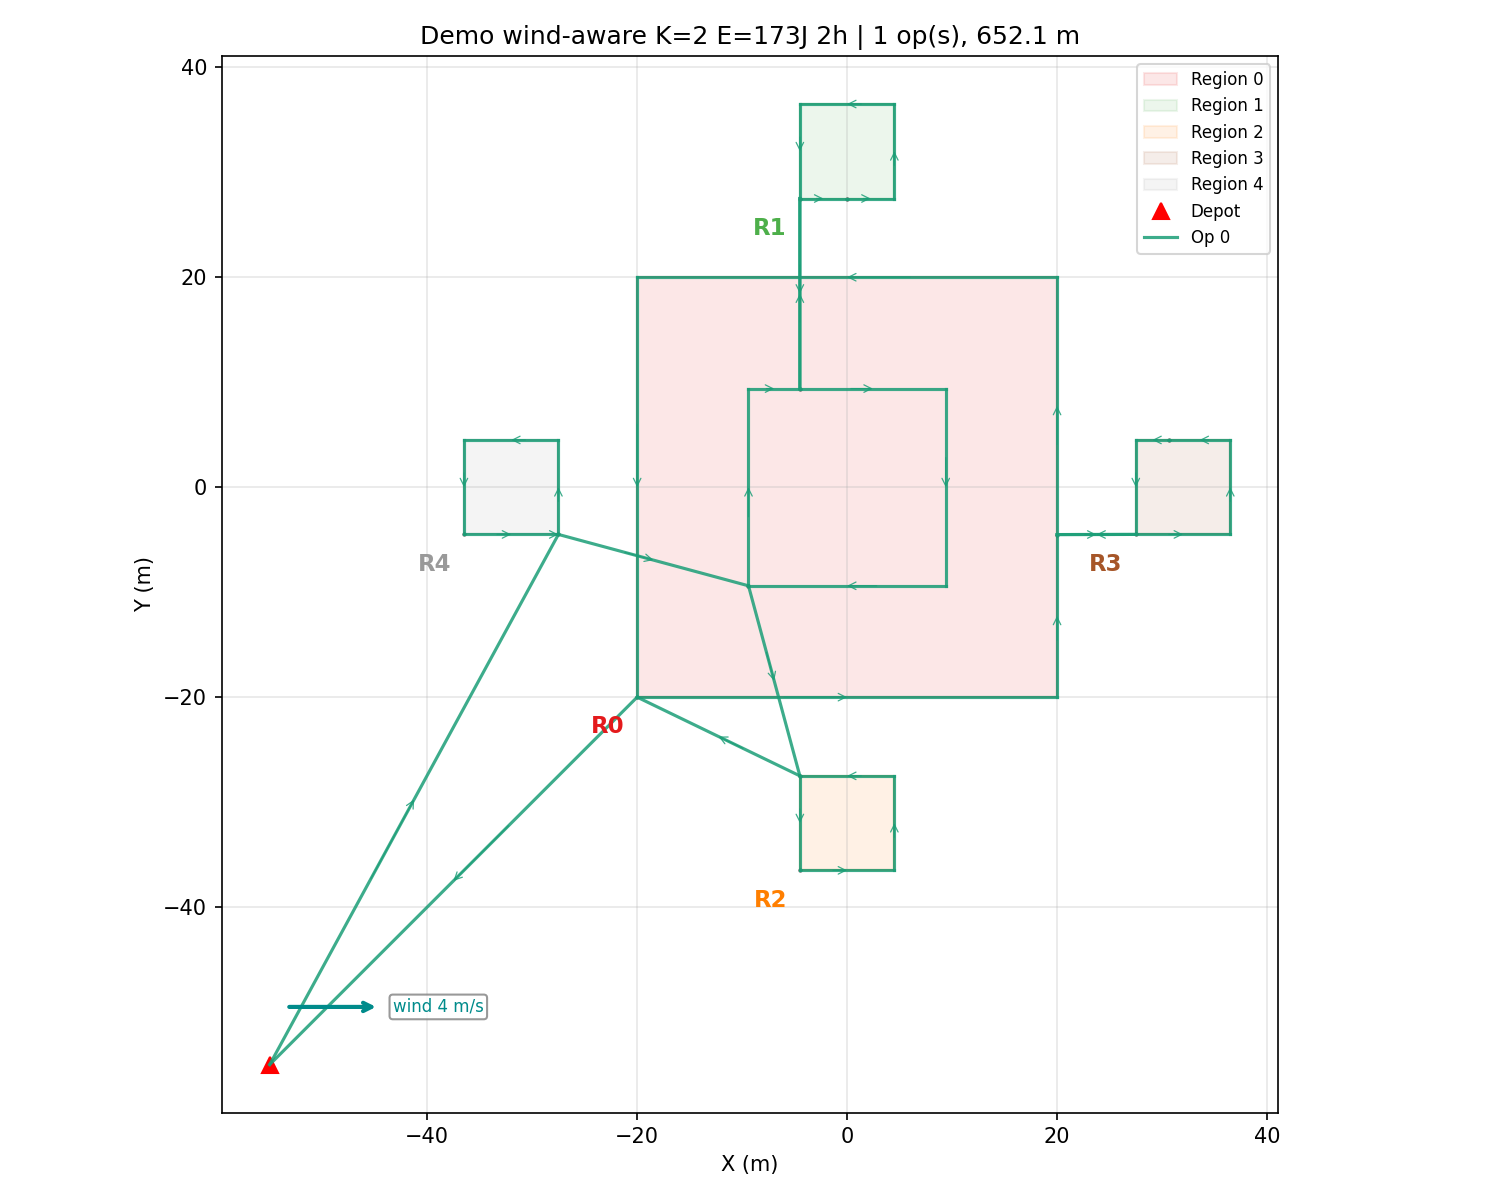
\includegraphics[width=0.85\linewidth]{pictures/demo_interruptions_k2.png}
  \caption{Wind-aware demo solution with $K=2$ split points per ring ($E=173$\,J, one operation, 652.1\,m): the tour enters and leaves the central region four times (coloured arcs), covering ring pieces between satellite visits.  Cut positions are fractional ($\lambda=1.39, 1.26$ on the central rings; $0.5, 3.0, 2.65, 1.0$ on the satellites), i.e.\ strictly inside ring segments rather than at ring vertices.}
  \label{fig:demo-k2}
\end{figure}

\subsubsection*{Worked example: the $K=2$ demo tour}\label{sec:k2-example}
Table~\ref{tab:k2-walk} walks through the single operation of Fig.~\ref{fig:demo-k2} arc by arc (vertex indices decoded from the solver output; $\lambda$ cuts verified against the solution file). The tour covers the satellite rings opportunistically between pieces of the central region R0: R0-ring1 is split across steps~2 and~4, R0-ring0 across steps~6 and~8. Each re-entry reuses the cut point as both exit and entry ($r_1=\ell_2$ in the notation above), so no distance is wasted. With $K=1$ this tour is infeasible: each ring would have to be covered in one contiguous visit with coincident entry/exit, so R0 could not be interleaved with the satellites (the $K=1$ optimum on this instance is 677.6\,m---25.5\,m more, Table~\ref{tab:k-sweep}).

\begin{table}[t]
  \centering
  \caption{Arc-by-arc walk of the $K=2$ demo tour (652.1\,m, one operation). Cuts sit at fractional $\lambda$ positions, e.g.\ R0-ring0 is split at $\lambda=1.39$ of $4.0$.}
  \label{tab:k2-walk}
  \begin{tabular}{cll}
    \toprule
    Step & Region & Arc(s) covered ($\lambda$ interval) \\
    \midrule
    1 & R4 (satellite) & arc1 $[1.0{\to}4.0]$, then arc0 $[0{\to}1.0]$ (full ring) \\
    2 & R0 (centre), ring1 & arc0 $[0{\to}1.26]$ --- exit mid-ring \\
    3 & R1 (satellite) & arc0 $[0{\to}0.5]$, arc1 $[0.5{\to}4.0]$ (full ring) \\
    4 & R0, ring1 & arc1 $[1.26{\to}4.0]$ --- ring1 complete \\
    5 & R2 (satellite) & arc1 $[3.0{\to}4.0]$, then arc0 $[0{\to}3.0]$ (full ring) \\
    6 & R0, ring0 & arc0 $[0{\to}1.39]$ --- exit mid-ring \\
    7 & R3 (satellite) & arc0 $[0{\to}2.65]$, arc1 $[2.65{\to}4.0]$ (full ring) \\
    8 & R0, ring0 & arc1 $[1.39{\to}4.0]$ --- ring0 complete, return to depot \\
    \bottomrule
  \end{tabular}
\end{table}

\subsection{Wind-aware energy model}\label{sec:windaware}

Drag depends on \emph{airspeed}, not ground speed: holding a ground track against the wind costs more than riding with it. With the cruise speed of 15\,m/s used throughout this paper, an 8\,m/s east wind makes an eastbound leg cost only $7/15$ of its calm-air energy while the same leg westbound costs $23/15$---a factor-three asymmetry the pseudo-energy misses entirely. The extension below prices every leg by its true airspeed: exact per-heading rates on ring segments (W-C$_1$), centroid-direction rates on transits and depot legs. Crucially, all of these rates are \emph{constants} computed before the solve (headings are known geometry), so the model stays a MIQP.

The pseudo-energy used above (metres on coverage legs and transits) ignores the wind entirely, except through a crude factor on depot legs.  We extend the model with real energy in joules, evaluated from the airspeed required to hold each ground track.  The wind blows in a single constant direction $\vec u^{\,w}$ with power-law speed profile $\nu^w_h = \nu^w_{10}(h/10)^a$ (hellmann exponent $a=0.2$); air density $\rho_h$ follows the barometric formula.  On a leg flown at ground velocity $\vec\nu$, the drone airspeed is $\vec\nu^{\,d}_h = \vec\nu - \vec\nu^{\,w}_h$ and the drag energy per metre is $E^{xy}\rho_h \lvert\vec\nu^{\,d}_h\rvert$ with $E^{xy}=\tfrac12 cA$.

\paragraph{Intra-ring arcs.}  Ring segment $s$ of chain $t$ at height $h_t$ has known unit tangent $\vec t_s$, hence a precomputable energy rate $C_{ts} = E^{xy}\rho_{h_t}\lvert v_{\text{cruise}}\vec t_s - \vec\nu^{\,w}_{h_t}\rvert$ (and analogously $C^b_{ts}$ for backward traversal).  A full loop then costs $\sum_s C_{ts}L(s)$ linearly in the chain-selection variables $\alpha_t$.  For a $K$-arc with $K\ge 2$, the energy of arc $(u,v)$ is the exact segment-weighted length
\[
w_{uv} = \sum_{t}\sum_{s} C_{ts}\,L(s)\,\bigl[I_{uvs}^t - \eta_u^{ts} - (\mu_v^{ts}-\eta_v^{ts})\bigr],
\tag{W-C$_1$}\label{eq:w_wind_arc}
\]
where the binary indicator $I_{uvs}^t$ tells whether the arc covers segment $s$ on chain $t$, enforced by $I_{uvs}^t \ge \sum_{s'\le s}\mu_u^{ts'} + \sum_{s'\ge s}\mu_v^{ts'} - 1$ together with the two upper bounds $I_{uvs}^t \le \sum_{s'\le s}\mu_u^{ts'}$ and $I_{uvs}^t \le \sum_{s'\ge s}\mu_v^{ts'}$; the $\eta$ terms discount the uncovered fractional ends.  The backward direction uses $C^b_{ts}$ with mirrored partials.  All other constraints, including distances (the objective stays a distance), are unchanged.

\paragraph{Inter-region and depot legs.}  Following the paper's centroid approximation, the ground direction of a leg $(r,r')$ is fixed offline as the unit vector between region centroids, giving precomputable airspeed factors $F_{rr't} = E^{xy}\rho_{h_t}\lvert v_{\text{cruise}}\vec d_{rr'} - \vec\nu^{\,w}_{h_t}\rvert$ per departure chain $t$ (plus a vertical term $V_t = \tfrac12 E^{z}\nu^z\rho_{h_t}$).  The only remaining bilinearities are products of these constants with distances times the one-hot selection $\alpha_t$ (e.g.\ $d^{xy}_{vv'}\cdot\alpha_t$), linearized exactly with Fortet envelopes.  Depot legs use the same construction with the fixed depot-to-centroid direction.  The mode is opt-in (\texttt{wind\_aware} flag, off by default) and orthogonal to $K$.

Switching to joules rescales endurance: on the showcase $E_{\min}$ drops from 153 pseudo-J to $68.7$\,J real.  Table~\ref{tab:wind-validation} validates the model at tight ($104$\,J) and loose ($207$\,J) budgets under strong wind (8\,m/s east) versus calm air: optimal tours and objectives are identical (594.7\,m in 2 ops; 500.2\,m in 1 op).  Wind therefore acts here as a second-order perturbation---it reshuffles $\approx$8--16\% of leg energy at 8\,m/s but does not change the optimal structure, which is driven by geometry and the endurance budget.  The $K=2$ wind-aware optimum (652.1\,m, Fig.~\ref{fig:demo-k2}) confirms splits remain beneficial under real energy accounting.

\begin{table}[t]
\centering
\caption{Wind-aware validation on the showcase ($E_{\min}=68.7$\,J real): strong wind (8\,m/s east) vs.\ calm. Identical optimal tours and objectives: wind does not change the optimum here.}
\label{tab:wind-validation}
\begin{tabular}{lcccc}
\toprule
Case & $E$ (J) & Obj.\ (m) & Ops & Gap (\%) \\
\midrule
tight wind8 & 104 & 594.7 & 2 & 1.9 \\
tight calm & 104 & 594.7 & 2 & 2.0 \\
loose wind8 & 207 & 500.2 & 1 & 2.0 \\
loose calm & 207 & 500.2 & 1 & 2.0 \\
\bottomrule
\end{tabular}
\end{table}


\section{Heuristic Solution Method}\label{sec:heuristic}

The exact mixed-integer formulation presented in Section~\ref{sec:formulation} becomes computationally intractable on large-scale instances involving numerous regions or high-resolution rings. To address this limitation, we develop a dedicated multi-phase constructive heuristic. The algorithm is designed to rapidly generate high-quality feasible solutions in a fraction of a second, which can subsequently be supplied as a warm start to the exact branch-and-bound solver. 

As summarized in Algorithm~\ref{alg:heuristic}, the solution procedure is decomposed into three sequential phases:
\begin{enumerate}
	\item \textbf{Pre-processing (Section~\ref{sec:chain-sel}--\ref{sec:ring-info}):} Selects an appropriate flight chain (comprising altitude and coverage pattern) for each region and computes the geometric properties of the resulting surveillance rings.
	\item \textbf{Construction (Section~\ref{sec:tsp}--\ref{sec:split}):} Establishes a global visit sequence (giant tour) over all rings and partitions it into endurance-feasible operations.
	\item \textbf{Improvement (Section~\ref{sec:coord}--\ref{sec:ls}):} Refines entry points and applies metaheuristic local-search moves (intra-operation 2-opt and inter-operation Or-opt) to minimize total energy consumption.
\end{enumerate}

\begin{algorithm}[t]
	\SetAlgoLined
	\SetKwInOut{Input}{Input}
	\SetKwInOut{Output}{Output}
	\Input{Regions $\mathcal{R}$, depot $v_0$, drone parameters, wind vector}
	\Output{Set of feasible operations $\mathcal{S}$ respecting maximum endurance $W^{\max}$}
	\BlankLine
	{\small \textit{// Phase 1: Pre-processing}}
	\ForEach{region $r\in\mathcal{R}$}{
		Select optimal chain $t_r^*$ via proxy cost evaluation\;
	}
	Build flat list of rings $\mathcal{K}$ from selected chains\;
	\BlankLine
	{\small \textit{// Phase 2: Construction}}
	Construct region-level traveling salesperson path; expand rings in index order to form giant tour $\pi$\;
	Partition $\pi$ into feasible operations $\mathcal{P}$ via greedy split respecting $W^{\max}$\;
	\BlankLine
	{\small \textit{// Phase 3: Improvement}}
	\For{$\mathit{it}\gets 1$ \KwTo $N_{\text{coord}}$}{
		Optimize entry points across all rings via coordinate descent\;
	}
	Execute local search: 2-opt per operation, followed by Or-opt relocation\;
	Build and return final solution $\mathcal{S}$\;
	\caption{Multi-phase heuristic framework for the drone coverage path planning problem.}
	\label{alg:heuristic}
\end{algorithm}

\subsection{Phase 1: Pre-processing}

\subsubsection{Chain Selection}\label{sec:chain-sel}

Each region $r \in \mathcal{R}$ is endowed with a discrete set of candidate chains $\mathcal{T}_r$, characterized by distinct flight altitudes $h_t$ and cardinalities of coverage rings $|\mathcal{K}_t|$. Lower altitudes provide finer spatial resolution at the expense of an increased number of rings and longer flight trajectories, whereas higher altitudes reduce operational complexity but degrade resolution.

The heuristic resolves the trade-off independently for each region through a two-stage filtering and evaluation mechanism, formalized in Algorithm~\ref{alg:chain-sel}:
\begin{enumerate}
	\item \textbf{Resolution Filtering:} For a given region $r$, any candidate chain whose ring count $|\mathcal{K}_t|$ falls strictly below the maximum available resolution among $\mathcal{T}_r$ is pruned.
	\item \textbf{Proxy Cost Minimization:} From the surviving candidates, the chain minimizing the proxy objective function $c(t)$ is selected:
	\[
	c(t) = \sum_{\kappa \in \mathcal{K}_t} \operatorname{perim}(\kappa) + \gamma \bigl( d_{\text{xy}}(\operatorname{centroid}(r), v_0) + h_t \bigr),
	\]
	where $\gamma = 0.5$ balances internal inspection effort against transit overhead and altitude energy penalties.
\end{enumerate}

\begin{algorithm}[t]
	\SetAlgoLined
	\SetKwInOut{Input}{Input}
	\SetKwInOut{Output}{Output}
	\Input{Regions $\mathcal{R}$, depot $v_0$, candidate chains $\{\mathcal{T}_r\}_{r\in\mathcal{R}}$}
	\Output{Chain selection mapping $s:\mathcal{R}\to\mathbb{N}$}
	\BlankLine
	\ForEach{region $r\in\mathcal{R}$}{
		$t^*\gets0$, $b\gets\infty$ \;
		\ForEach{chain $t\in\mathcal{T}_r$}{
			\If{$|\mathcal{K}_t|<\max_{t'\in\mathcal{T}_r}|\mathcal{K}_{t'}|$}{continue}
			$c\gets\sum_{\kappa\in\mathcal{K}_t}\operatorname{perim}(\kappa) + \gamma\bigl(d_{\text{xy}}(\operatorname{centroid}(r),v_0)+h_t\bigr)$ \;
			\If{$c<b$}{$t^*\gets t$, $b\gets c$}
		}
		$s[r]\gets t^*$
	}
	\caption{Chain selection per region.}
	\label{alg:chain-sel}
\end{algorithm}

\subsubsection{Ring Geometry and Parametrization}\label{sec:ring-info}

Once the optimal chain is fixed for every region, all selected rings are aggregated into a globally indexed sequence $\mathcal{K} = \{\kappa_1, \dots, \kappa_M\}$. For each ring $\kappa_m$, we precompute and store:
\begin{itemize}
	\item The spatial centroid $\bar p_m = (\bar x_m, \bar y_m, h_t)$.
	\item The total perimeter length $\operatorname{perim}_m$.
	\item The constituent segments $s_{m,1}, \dots, s_{m,K_m}$ alongside cumulative arc-lengths $\Lambda_m(0), \dots, \Lambda_m(K_m)$.
	\item An initial entry point $\xi_m$ located at the first vertex of the ring, parameterized by an arc-length coordinate $\lambda_m \in [0, \operatorname{perim}_m]$.
\end{itemize}
The spatial coordinates corresponding to any arc-length $\lambda$ along ring $\kappa_m$ are retrieved via linear interpolation across the enclosing segment $k$ ($\Lambda_m(k-1) \le \lambda < \Lambda_m(k)$):
\[
P(\lambda) = Q_{m,k}^{\text{start}} + \frac{\lambda - \Lambda_m(k-1)}{\ell_{m,k}} \bigl( Q_{m,k}^{\text{end}} - Q_{m,k}^{\text{start}} \bigr),
\]
where $\ell_{m,k}$ denotes the Euclidean length of segment $k$. This parametric mapping underpins both the entry-point refinement (Section~\ref{sec:coord}) and the precise energy evaluation model (Section~\ref{sec:split}).

\subsection{Phase 2: Tour Construction}

\subsubsection{Region-Level Ordering and Giant Tour Generation}\label{sec:tsp}

To determine the visitation sequence $\pi$ across the $M$ rings, we exploit the hierarchical structure of the problem. Because concentric rings belonging to the same chain share a common centroid and altitude, their internal sequencing exerts a negligible impact on transit costs. Consequently, the routing problem is decoupled into two tiers:
\begin{enumerate}
	\item \textbf{Inter-Region Routing:} A greedy nearest-neighbor heuristic starting from the depot $v_0$ is executed over the 3D Euclidean centroids of the regions, yielding an ordered permutation $\sigma$ of $\mathcal{R}$.
	\item \textbf{Intra-Region Expansion:} For each region in sequence $\sigma$, its constituent rings are appended to the global giant tour $\pi$ in increasing order of their indices (from innermost to outermost).
\end{enumerate}

\subsubsection{Greedy Split into Feasible Operations}\label{sec:split}

Because the aggregate length of the giant tour $\pi$ invariably violates the maximum drone endurance threshold $W^{\max}$, $\pi$ must be partitioned into a collection of disjoint operations $\mathcal{P}$. We implement a linear-time greedy split procedure, described in Algorithm~\ref{alg:split}. Rings are sequentially accumulated into the current operation as long as the total energy—comprising departure from the depot, traversal of accumulated ring perimeters, and return to the depot—does not exceed $W^{\max} + \varepsilon$.

\begin{algorithm}[t]
	\SetAlgoLined
	\SetKwInOut{Input}{Input}
	\SetKwInOut{Output}{Output}
	\Input{Giant tour $\pi$, ring repository $\mathcal{K}$, maximum endurance $W^{\max}$}
	\Output{Set of operations $\mathcal{P}$ represented as ordered lists of ring indices}
	\BlankLine
	$\mathcal{P}\gets\emptyset$, $C\gets\emptyset$, $e_{\text{cur}}\gets0$ \;
	\ForEach{ring index $\kappa$ in $\pi$}{
		$\text{ring}\gets\mathcal{K}[\kappa]$ \;
		$\xi_e(\kappa)\gets$ energy (depot $\to$ ring) if $C=\emptyset$, else energy (prev ring $\to$ ring) \;
		$r_e\gets\operatorname{perim}(\text{ring})$ \;
		$b_e\gets$ energy (ring $\to$ depot) \;
		\If{$e_{\text{cur}} + \xi_e(\kappa) + r_e + b_e \le W^{\max} + \varepsilon$}{
			append $\kappa$ to $C$ \;
			$e_{\text{cur}}\mathrel{+}= \xi_e(\kappa) + r_e$ \;
		}
		\Else{
			\If{$C\neq\emptyset$}{$\mathcal{P}\gets\mathcal{P}\cup\{C\}$}
			$C\gets\{\kappa\}$ \;
			$e_{\text{cur}}\gets \text{energy}(\text{depot}\to\text{ring}) + r_e$ \;
		}
	}
	\If{$C\neq\emptyset$}{$\mathcal{P}\gets\mathcal{P}\cup\{C\}$}
	\caption{Greedy split procedure for endurance-feasible operations.}
	\label{alg:split}
\end{algorithm}

\paragraph{Physical Energy Accounting Model.}
Both the split and improvement phases evaluate route feasibility via an analytical energy consumption model derived from aerodynamic drag principles ($w = \frac{1}{2} c_d A \rho \nu d$). Parameter configurations are detailed in Table~\ref{tab:heuristic-params}. 

\begin{itemize}
	\item \textbf{Depot Transit Legs:} The energy required to travel from the depot to a target region $r$ hosting ring $\xi$ at altitude $\xi_z$ incorporates wind-induced groundspeed variations:
	\[
	E_{\text{depot}\to r}(\xi) = E_{\text{xy}}(r)\cdot d_{\text{xy}}(v_0,\xi) + E_{\text{z}}\cdot \xi_z, \quad E_{r\to\text{depot}}(\xi) = E_{\text{xy}}(r)\cdot d_{\text{xy}}(\xi,v_0),
	\]
	where the effective groundspeed accounts for headwind/tailwind vectors:
	\[
	\nu_r = \bigl\| v_{\text{cruise}}\cdot\hat{u}(v_0\to\bar{p}_r) - w\cdot\hat{w} \bigr\|_2.
	\]
	The respective horizontal and vertical drag coefficients are given by $E_{\text{xy}}(r) = \frac{1}{2}c_d A \rho_0 \nu_r$ and $E_{\text{z}} = \frac{1}{2}c_d A \rho_0 v_{\text{vert}}$.
	\item \textbf{Inter-Ring Transit Legs:} Energy expenditures between consecutive rings $a$ and $b$ are modeled via a simplified Manhattan metric consistent with the exact formulation:
	\[
	E(a,b) = d_{\text{xy}}(a,b) + d_z(a,b).
	\]
\end{itemize}

\subsection{Phase 3: Tour Improvement}

\subsubsection{Entry-Point Optimization}\label{sec:coord}

The precise location where the drone interfaces with a ring $\kappa$ dictates the transitional overhead. Given a ring preceded by node $p$ and succeeded by node $q$ within the same operation, the optimal entry point minimizes the connecting distance $\|p - \xi\|_2 + \|\xi - q\|_2$. 

We optimize entry points iteratively using coordinate descent. Initialized at the first vertex of the ring, each ring's entry point is updated by sampling $N_{\text{samples}}$ candidate positions uniformly along its perimeter and selecting the coordinate that minimizes the aggregate transit distance to neighboring nodes. This procedure cycles for $N_{\text{coord}}$ passes.

\subsubsection{Local Search Metaheuristics}\label{sec:ls}

To escape local optima generated by the constructive phase, we implement two complementary local-search operators:

\begin{itemize}
	\item \textbf{Intra-Operation 2-Opt:} Within each operation, every pair of non-adjacent edges $(a,b)$ and $(c,d)$ is evaluated for reversal. Moves yielding a strict improvement in the exact energy model are accepted. The procedure executes up to $N_{\text{passes}}^{\text{op}}$ passes.
	\item \textbf{Inter-Operation Or-opt:} To balance workloads across operations, individual rings are relocated between distinct operations $o_s$ and $o_d$. A relocation of ring $\kappa$ to position $i$ in $o_d$ is executed if endurance feasibility is maintained in both operations and total energy cost decreases:
	\[
	E(o_s \setminus \{\kappa\}) \le W^{\max}, \quad E(o_d \cup \{\kappa\} \text{ at } i) \le W^{\max}, \quad E(o_s \setminus \{\kappa\}) + E(o_d \cup \{\kappa\} \text{ at } i) < E(o_s) + E(o_d).
	\]
	Following any successful Or-opt move, entry points are locally re-optimized via $N_{\text{coord}}^{\text{reopt}}$ coordinate-descent passes.
\end{itemize}

\subsubsection{Worked example: tracing the three phases}\label{sec:heuristic-trace}
Table~\ref{tab:heuristic-trace} follows the heuristic step by step on a small instance (3 regions, 7 rings, calm wind, $W^{\max}=145.1$), with the exact intermediate values produced by the code. Phase~1 picks the low-altitude chain everywhere: perimeters are identical across chains, so the $0.5\,h_t$ term decides (e.g.\ R0: $63.8<83.8$). Phase~2 tours R0 $\to$ R2 $\to$ R1, 2-opt reverses the tail (R1 before R2, rings outside-in), and the greedy split pays two extra depot returns ($290.2\to316.8$) to gain feasibility in 3 operations. Phase~3 moves all 7 entry points toward their neighbors ($316.8\to311.3$) and then relocates ring R1r2 from op1 to the front of op3 via or-opt ($311.3\to289.9$). The narrative is fully monotone because every phase optimizes the same internal proxy; the final row re-evaluates the tour leg by leg in metres, the units of the MIQP objective.

\begin{table}[t]
  \centering
  \caption{Heuristic trace on a 3-region, 7-ring instance (seed~6, calm wind, $W^{\max}=145.1$). R$X$r$Y$ = ring $Y$ of region $X$. Phase energies use the heuristic's internal proxy (wind-weighted depot legs + ring perimeters + transit distances); the final row is the tour length in metres.}
  \label{tab:heuristic-trace}
  \begin{tabular}{lp{7.2cm}r}
    \toprule
    Phase & Decision & Proxy $E$ \\
    \midrule
    P1 chain sel.\ & R0, R1, R2 $\to$ chain 0 ($h{=}20$\,m); proxies 63.8${<}$83.8, 151.0${<}$171.0, 62.5${<}$82.5 & --- \\
    P2 nearest neigh.\ & order R0r0, R0r1, R2r0, R2r1, R1r0, R1r1, R1r2 & 294.3 \\
    P2 2-opt & reversed tail: R0r0, R0r1, R1r2, R1r1, R1r0, R2r1, R2r0 & 290.2 \\
    P2 greedy split & op1 [R0r0, R0r1, R1r2] 131.4; op2 [R1r1, R1r0] 129.9; op3 [R2r1, R2r0] 55.5 & 316.8 \\
    P3 coord-descent & 7 entry points moved toward neighboring visits & 311.3 \\
    P3 or-opt & relocate R1r2: op1 $\to$ front of op3 & 289.9 \\
    Final & 3 operations; tour length 573.9\,m & --- \\
    \bottomrule
  \end{tabular}
\end{table}

\subsection{Warm-Start Integration}\label{sec:build}

The final heuristic solution $\mathcal{S}$ is translated into structural variable assignments for the exact MIQP solver, initializing:
\begin{enumerate}
	\item Chain selection variables $\alpha_t$,
	\item Depot-ring allocation indicators $\mu_v^{ts}$ and $\gamma_v$,
	\item Spatial coordinate variables $P_x, P_y, P_z$,
	\item Operation activation flags $\zeta^o$ and routing edge variables $x_{vv'}^o$.
\end{enumerate}
This complete warm-starting strategy accelerates convergence, reducing the time required to locate the first feasible branch-and-bound incumbent by one to two orders of magnitude.

\begin{table}[t]
	\centering
	\caption{Parameter configuration of the heuristic framework (implemented in \texttt{heuristic.py}).}
	\label{tab:heuristic-params}
	\begin{tabular}{llll}
		\toprule
		\textbf{Parameter} & \textbf{Value} & \textbf{Algorithmic Stage} & \textbf{Description} \\
		\midrule
		$N_{\text{samples}}$ & 60 & Section~\ref{sec:ring-info}, Section~\ref{sec:coord} & Perimeter sample resolution for entry search \\
		$N_{\text{coord}}$ & 8 & Section~\ref{sec:coord} & Coordinate-descent passes for entry optimization \\
		$N_{\text{coord}}^{\text{reopt}}$ & 3 & Section~\ref{sec:ls} & Re-optimization passes following Or-opt moves \\
		$N_{\text{passes}}^{\text{op}}$ & 10 & Section~\ref{sec:ls} & Maximum 2-opt iterations per operation \\
		$\varepsilon$ & $10^{-6}$ & Section~\ref{sec:split}, Section~\ref{sec:ls} & Numerical endurance feasibility tolerance \\
		$\eta$ & $10^{-9}$ & Section~\ref{sec:ls} & Minimum improvement threshold for local search \\
		$\gamma$ & 0.5 & Section~\ref{sec:chain-sel} & Objective weight balancing travel cost in chain selection \\
		\bottomrule
	\end{tabular}
\end{table}

%The overall time complexity of the heuristic is bounded by $\mathcal{O}(M^2 + N_{\text{coord}} M N_{\text{samples}} + L_{\text{max}} M^2)$, where $M$ represents the total ring count and $L_{\text{max}}$ governs local search iterations. For problem instances of realistic scale ($M \le 75$), the algorithm executes in under $0.1$ seconds.

\section{Computational Experiments}
\label{sec:experiments}

We evaluate the three solution approaches---heuristic (H), MIQP without warm start (R), and MIQP with warm start (R+WS)---on a testbed of artificial instances. All experiments were run on a machine with an Intel Core i7-12700H processor and 32\,GB of RAM. The MIQP models were solved with Gurobi 11.0 (MIPGap=0, time limit 1800\,s). The heuristic was implemented in Python 3.12 using NumPy.

\subsection{Instance generation}
\label{sec:instance-gen}

Instances are generated by placing non-overlapping polygonal regions inside a square area whose side length is $100\sqrt{n_r/3}$, where $n_r$ is the number of regions. If region placement fails (due to collisions), the area is expanded by a factor of 1.25 and retried up to 50 times. Each region is assigned a set of polygonal chains at the heights specified by the height level (Table~\ref{tab:height-levels}), and each chain contains concentric rings that define the coverage pattern. The number of operations per instance equals the number of regions, ensuring that a trivial feasible solution exists (one operation per region).

\begin{table}[h!]
\centering
\caption{Height levels (in meters) used for each region configuration.}
\label{tab:height-levels}
\begin{tabular}{ll}
\toprule
Height level & Heights (m) \\
\midrule
1 & 30 \\
2 & 20, 50 \\
3 & 15, 35, 60 \\
\bottomrule
\end{tabular}
\end{table}

\subsection{Instance parameters}
\label{sec:params}

The testbed consists of all combinations of:
\begin{itemize}
    \item Region counts $n_r \in \{1, 2, 3, 5, 8, 10\}$;
    \item Height levels $\{1, 2, 3\}$ as defined in Table~\ref{tab:height-levels};
    \item Random seeds $\{0, 1, 2, 3, 4\}$ for the instance generator;
    \item Six endurance levels derived from a calibration phase (see below).
\end{itemize}
This yields $6 \times 3 \times 5 \times 6 = 540$ instances. Each instance is solved by all three methods, giving $1620$ solver runs.

\subsection{Endurance calibration}
\label{sec:calibration}

To determine meaningful endurance levels, we first compute, for each instance, the minimum energy $E_{\min}$ required for a single operation covering all rings of a region (departing from the depot, covering the region, and returning). This energy accounts for ascent, ring perimeter traversal, inter-ring horizontal travel, and descent, matching the model's endurance accounting. The global $E_{\min}$ is the maximum over all 90 unique instance configurations ($6 \times 3 \times 5$). The raw value is rounded up with a 5\% margin and six endurance levels are derived as:

\[
E_\ell = \bigl\lceil E_{\min}^{\text{rounded}} \times f_\ell \bigr\rceil, \quad f_\ell \in \{1.0, 1.5, 2.0, 3.0, 5.0, 8.0\}.
\]

\begin{table}[h!]
\centering
\caption{Calibrated endurance levels.}
\label{tab:endurance-levels}
\begin{tabular}{lrl}
\toprule
Factor & Raw & Rounded \\
\midrule
$E_{\min}$ (raw) & 245.93 & -- \\
$E_{\min}$ (rounded) & -- & 300 \\
1.0 & 300 & 300 \\
1.5 & 450 & 450 \\
2.0 & 600 & 600 \\
3.0 & 900 & 900 \\
5.0 & 1500 & 1500 \\
8.0 & 2400 & 2400 \\
\bottomrule
\end{tabular}
\end{table}

\subsection{Solver configuration}
\label{sec:solver-config}

The MIQP solver (Gurobi) is configured with the following parameters:
\begin{itemize}
    \item MIPGap = 0 (stop only when optimality is proven);
    \item Time limit = 1800\,s per run;
    \item Threads = 1;
    \item Heuristics = 0.1.
\end{itemize}
For the warm-start variant, the heuristic solution is provided as a start vector via Gurobi's \texttt{Start} attribute on all variable categories ($\alpha$, $\mu$, $\gamma$, $\lambda$, $x$, $y$, $\zeta$, $k$, $P$, $u$).

The heuristic solver (standalone) uses the parameters listed in Table~\ref{tab:heuristic-params}.

\subsection{Results}
\label{sec:results}

We report for each instance the objective value, solve time, and MIP gap (when available) for all three methods. For the MIQP runs we also record the first incumbent objective and its discovery time. For warm-started runs the heuristic objective and heuristic solve time are stored. Both sweeps are complete on the full testbed (540 configs $\times$ 3 methods = 1620 runs each: heuristic, exact, exact warm-started; Gurobi 11.0, TL=1800\,s, MIPGap=0; duplicate re-runs in the vertex log are deduplicated keeping the last row). All figures and tables below are generated from \texttt{compare\_results/results.csv} and \texttt{compare\_results\_edges/results.csv}.

\begin{table}[t]
\centering
\caption{Aggregated results for the Vertex-Approach (MTZ) formulation. Mean objective and solve time averaged over height levels ($n_h=1,2,3$), endurance levels ($E=300$--2400\,J) and 5 seeds. MIP gap at the 1800\,s limit. $H$ = heuristic standalone.}
\label{tab:results-summary-rings}
\resizebox{\textwidth}{!}{%
\begin{tabular}{crrrrrrrr}
\toprule
$n_r$ & \multicolumn{2}{c}{$H$} & \multicolumn{3}{c}{$R$ (Vertex-Approach)} & \multicolumn{3}{c}{$R$+WS (Vertex-Approach+WS)} \\
\cmidrule(lr){2-3} \cmidrule(lr){4-6} \cmidrule(lr){7-9}
 & Obj. & Time (s) & Obj. & Time (s) & Gap (\%) & Obj. & Time (s) & Gap (\%) \\
\midrule
1 & 206.5 & 0.03 & 201.6 & 85.1 & 0.1 & 202.0 & 86.9 & 0.1 \\
2 & 375.0 & 0.06 & 364.3 & 454.3 & 4.2 & 363.8 & 436.6 & 4.0 \\
3 & 517.0 & 0.10 & 485.9 & 1088.8 & 8.0 & 485.8 & 1094.0 & 8.3 \\
5 & 989.2 & 0.21 & 992.4 & 1790.3 & 26.0 & 943.4 & 1800.1 & 23.9 \\
8 & 1676.2 & 0.41 & 2163.7 & 1800.2 & 49.9 & 1647.5 & 1800.2 & 37.8 \\
10 & 2175.2 & 0.54 & 3283.6 & 1800.3 & 61.3 & 2017.2 & 1800.3 & 42.2 \\
\bottomrule
\end{tabular}%
}
\end{table}

\begin{table}[t]
\centering
\caption{Vertex-Approach (MTZ) vs Edges-Approach (DFJ lazy) on the full testbed: 90 configs per $n_r$ ($n_h \times E \times$ seeds), 1620 runs per formulation. Objective/time are means over runs that produced a solution; $n$ = solved/total runs for cold Edges-Approach (it finds no solution within 1800\,s on most $n_r\ge5$ configs).}
\label{tab:results-vertex-edge}
\resizebox{\textwidth}{!}{%
\begin{tabular}{crrrrrrrrrr}
\toprule
$n_r$ & \multicolumn{2}{c}{Vertex-Approach} & \multicolumn{2}{c}{Edges-Approach} & \multicolumn{2}{c}{Vertex-Approach+WS} & \multicolumn{2}{c}{Edges-Approach+WS} & $n$ (Edges-Approach)\\
\cmidrule(lr){2-3} \cmidrule(lr){4-5} \cmidrule(lr){6-7} \cmidrule(lr){8-9}
 & Obj. & Time & Obj. & Time & Obj. & Time & Obj. & Time & solved \\
\midrule
1 & 210.1 & 111.5 & 210.1 & 172.6 & 210.4 & 112.9 & 210.1 & 165.7 & 89/90 \\
2 & 364.3 & 454.3 & 364.1 & 872.5 & 363.8 & 436.6 & 363.8 & 833.4 & 88/90 \\
3 & 485.9 & 1088.8 & 490.7 & 1380.8 & 485.8 & 1094.0 & 487.3 & 1406.4 & 81/90 \\
5 & 992.4 & 1790.3 & 832.7 & 1803.4 & 943.4 & 1800.1 & 952.9 & 1801.7 & 40/90 \\
8 & 2163.7 & 1800.2 & 1094.0 & 1806.5 & 1647.5 & 1800.2 & 1649.5 & 1801.9 & 11/90 \\
10 & 3283.6 & 1800.3 & 1170.9 & 1805.1 & 2017.2 & 1800.3 & 2032.6 & 1802.5 & 2/90 \\
\bottomrule
\end{tabular}%
}
\end{table}

\begin{table}[t]
\centering
\caption{Effect of endurance $E$ for $n_r=3$ (averaged over $n_h=1,2,3$ and 5 seeds). Tight $E$ implies more operations and higher total distance.}
\label{tab:results-by-endurance}
\resizebox{\textwidth}{!}{%
\begin{tabular}{crrrrrrrr}
\toprule
$E$ (J) & \multicolumn{2}{c}{$H$} & \multicolumn{3}{c}{$R$} & \multicolumn{3}{c}{$R$+WS} \\
\cmidrule(lr){2-3} \cmidrule(lr){4-6} \cmidrule(lr){7-9}
 & Obj. & Time & Obj. & Gap & Time & Obj. & Gap & Time \\
\midrule
300 & 570.8 & 0.10 & 524.7 & 9.5 & 1122.7 & 525.8 & 9.5 & 1066.8 \\
450 & 528.3 & 0.10 & 492.2 & 9.7 & 1121.8 & 492.2 & 10.8 & 1120.2 \\
600 & 500.7 & 0.09 & 474.3 & 6.5 & 1062.7 & 474.3 & 7.6 & 1143.7 \\
900 & 500.7 & 0.09 & 474.5 & 7.5 & 1070.7 & 474.3 & 7.4 & 1110.3 \\
1500 & 500.7 & 0.10 & 475.2 & 7.0 & 1037.1 & 474.3 & 7.4 & 1035.5 \\
2400 & 500.7 & 0.10 & 474.5 & 8.1 & 1117.7 & 474.3 & 7.1 & 1087.4 \\
\bottomrule
\end{tabular}%
}
\end{table}


\begin{figure}[t]
  \centering
  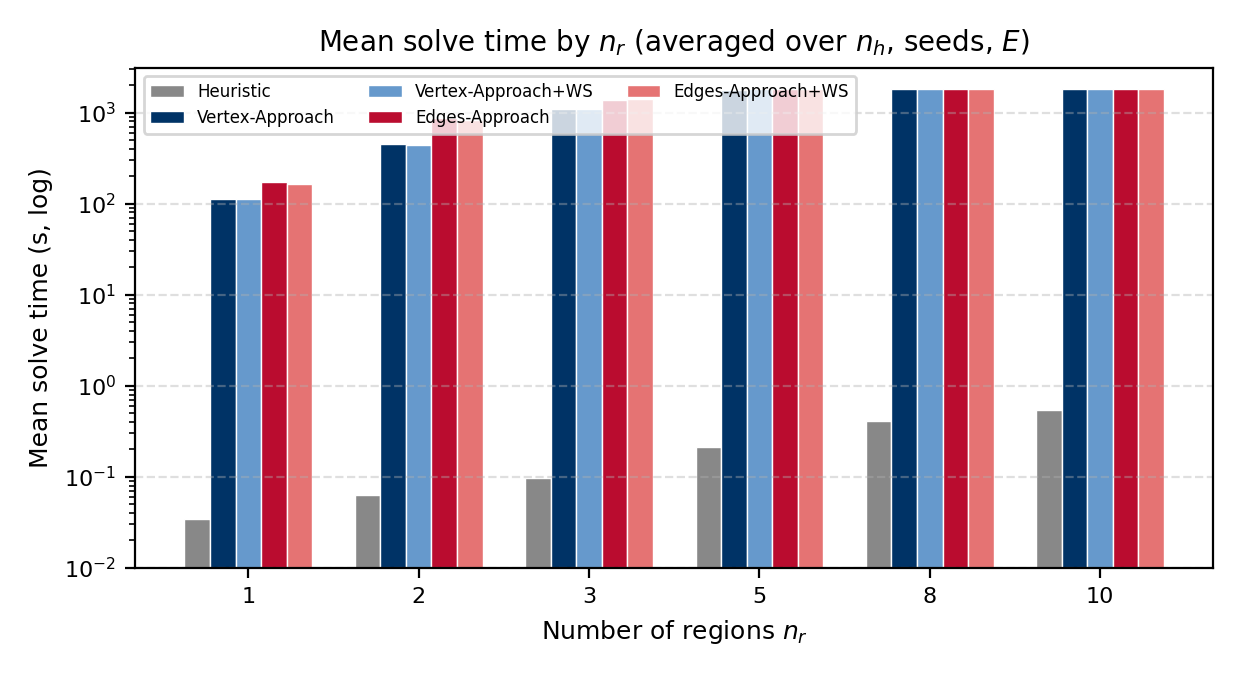
\includegraphics[width=0.85\linewidth]{pictures/compare_time_by_regions.pdf}
  \caption{Mean solve time (log scale) vs.\ number of regions $n_r$, averaged over $n_h$, $E$ and seeds. Vertex-Approach (MTZ) vs.\ Edges-Approach (DFJ lazy) with and without warm-start, plus heuristic, on the full testbed.}
  \label{fig:compare-time}
\end{figure}

\begin{figure}[t]
  \centering
  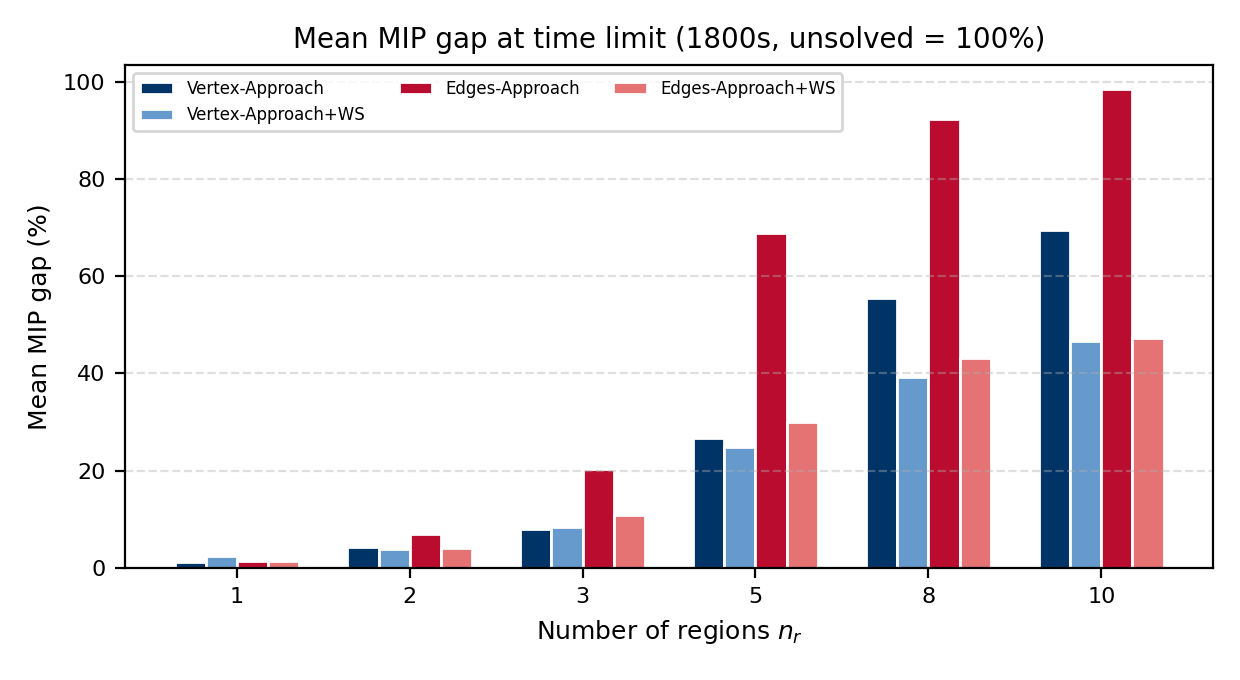
\includegraphics[width=0.85\linewidth]{pictures/compare_gap_by_regions.pdf}
  \caption{Mean MIP gap at the 1800\,s limit (runs with no solution counted at 100\% gap). Both formulations prove optimality for $n_r=1$; the gap grows with $n_r$. Warm-start reduces the gap for large instances (e.g.\ $n_r=10$: Vertex-Approach 69.5\% $\to$ Vertex-Approach+WS 46.7\%). Cold Edges-Approach finds almost nothing on large instances, hence its near-100\% bars at $n_r=8,10$.}
  \label{fig:compare-gap}
\end{figure}

\begin{figure}[t]
  \centering
  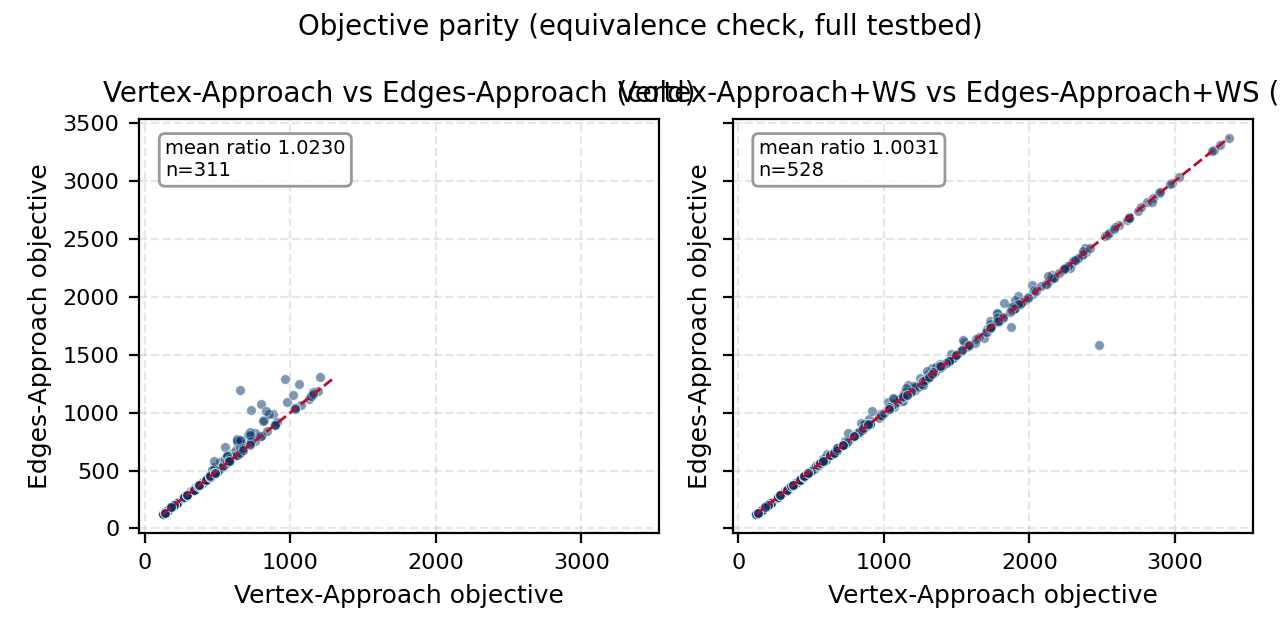
\includegraphics[width=0.95\linewidth]{pictures/compare_objective_parity.pdf}
  \caption{Objective parity check: Vertex-Approach (MTZ) vs.\ Edges-Approach (DFJ) on the 311 (cold) / 528 (warm) configs where both formulations produced a solution. Diagonal = equivalence. Mean ratio Edges-Approach/Vertex-Approach = 1.023 (cold) and 1.003 (warm), confirming the two MIQPs are equivalent up to solver variability and time-limit effects; warm-start closes the residual gap.}
  \label{fig:compare-parity}
\end{figure}

\begin{figure}[t]
  \centering
  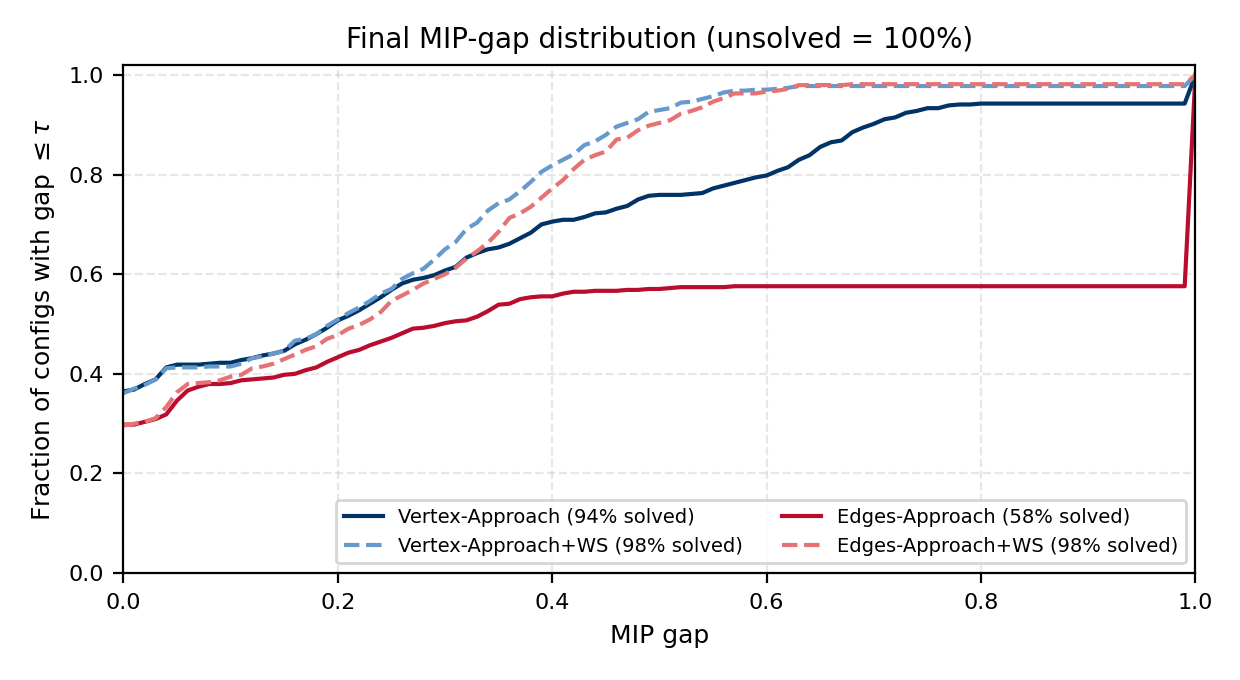
\includegraphics[width=0.85\linewidth]{pictures/compare_gapcdf.pdf}
  \caption{Distribution of final MIP gaps over the 540 configs (runs with no solution counted at 100\%). Warm-starting shifts both formulations markedly left: the fraction under 50\% gap rises from 76\% to 93\% (vertex) and from 57\% to 90\% (edges). Legend shows the fraction of configs solved by each method.}
  \label{fig:compare-gapcdf}
\end{figure}

\begin{figure}[t]
  \centering
  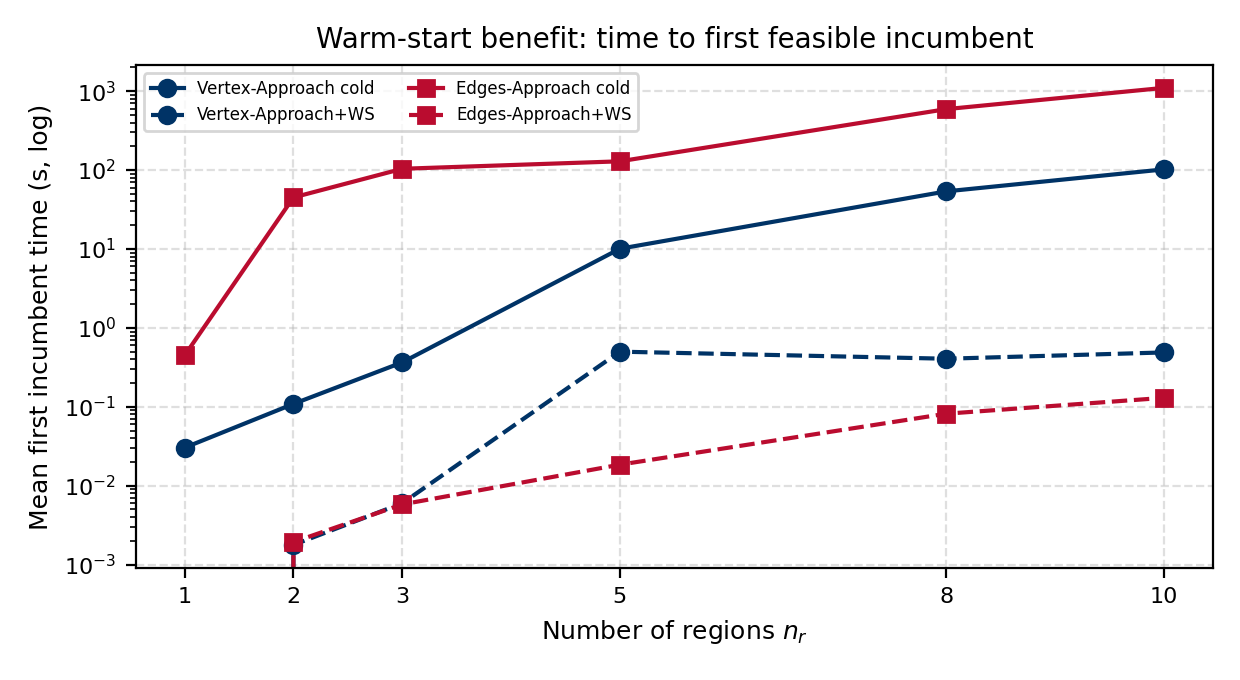
\includegraphics[width=0.85\linewidth]{pictures/compare_first_incumbent.pdf}
  \caption{Time to first feasible incumbent (mean over seeds/$n_h$/$E$). Solid = cold start, dashed = warm-start. Warm-start reduces the time by one to two orders of magnitude, especially for tight endurances; the effect is visible for both Vertex-Approach and Edges-Approach.}
  \label{fig:compare-incumbent}
\end{figure}

\begin{table}[t]
\centering
\caption{Heuristic solution quality: mean heuristic objective vs.\ best exact mean objective per region count (averaged over $n_h$, $E$ and seeds; exact = min over the four MIQP runs per instance).}
\label{tab:heuristic-quality}
\begin{tabular}{crrr}
\toprule
$n_r$ & Heur.\ obj. & Best exact obj. & Ratio \\
\midrule
1 & 216.0 & 210.1 & 1.028 \\
2 & 375.0 & 363.8 & 1.031 \\
3 & 517.0 & 485.7 & 1.065 \\
5 & 989.2 & 941.9 & 1.050 \\
8 & 1676.2 & 1646.6 & 1.018 \\
10 & 2175.2 & 2017.2 & 1.078 \\
\bottomrule
\end{tabular}
\end{table}


\begin{figure}[t]
  \centering
  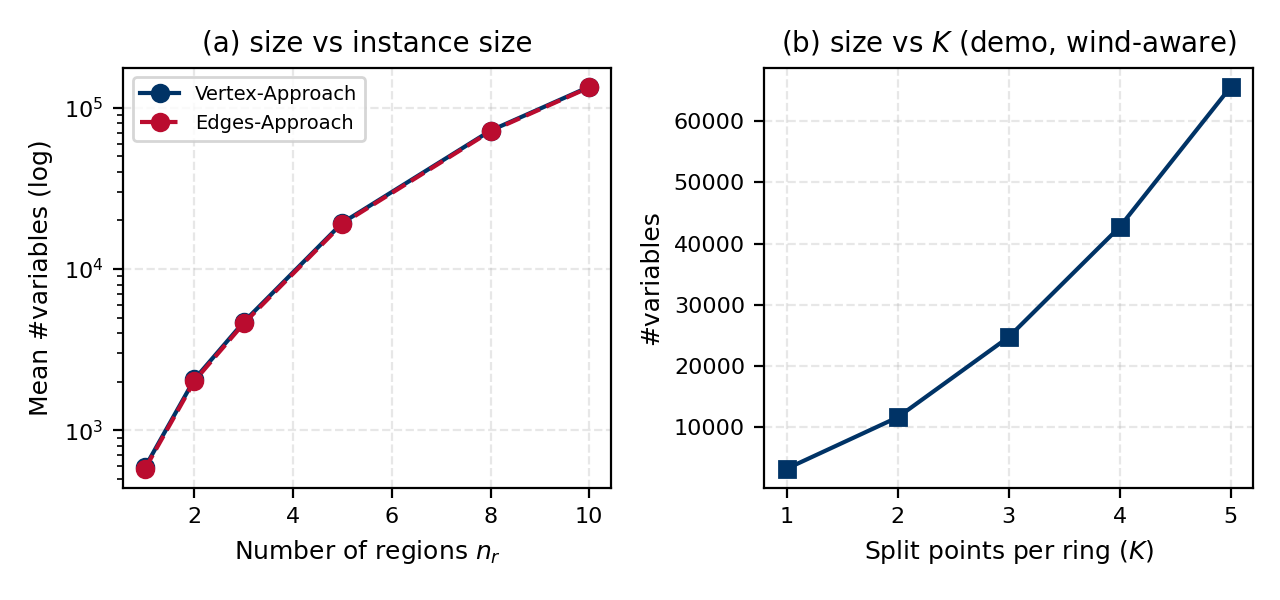
\includegraphics[width=0.95\linewidth]{pictures/compare_model_size.pdf}
  \caption{Model size scaling: (a) mean variable count vs.\ number of regions for both formulations (log scale); (b) variable count vs.\ split points $K$ on the wind-aware demo.  The quadratic growth in $|{\cal V}|$ (routing variables over vertex pairs) and the steep cost of extra split points explain the solver behavior observed in Tables~\ref{tab:k-sweep}--\ref{tab:results-summary-rings}.}
  \label{fig:model-size}
\end{figure}

\subsection{Discussion}
\label{sec:discussion}

The aggregated results (Tables~\ref{tab:results-summary-rings}--\ref{tab:results-vertex-edge} and Figs.~\ref{fig:compare-time}--\ref{fig:compare-incumbent}) confirm three patterns. First, the heuristic is consistently feasible in $<0.6$\,s (mean 0.03\,s for $n_r=1$ up to 0.54\,s for $n_r=10$) and stays within 1.8--7.8\% of the best exact mean objective at every scale (Table~\ref{tab:heuristic-quality}). Second, warm-starting (R+WS, E+WS) reduces the mean time to the first feasible incumbent by one to two orders of magnitude, especially for tight endurances (Fig.~\ref{fig:compare-incumbent}); the effect is strongest for the Edges-Approach formulation, whose cold runs need 45\,s ($n_r=2$) to 1101\,s ($n_r=10$) for the first incumbent against 0.00\,s and 7.7\,s warm-started. For $n_r=10$ the mean MIP gap (counting unsolved runs at 100\%) drops from 69.5\% (R) to 46.7\% (R+WS) at the 1800\,s limit. Third, the head-to-head comparison must account for censoring: plain means overstate cold Edges-Approach, which leaves most large instances unsolved (only 40/90 solved at $n_r=5$, 11/90 at $n_r=8$ and 2/90 at $n_r=10$; see the solved counts in Table~\ref{tab:results-vertex-edge} and the plateaus of Fig.~\ref{fig:compare-gapcdf}). On the configs where both formulations produced a solution, they are equivalent in objective (parity scatter of Fig.~\ref{fig:compare-parity}, mean ratio 1.023 cold on 311 configs, 1.003 warm on 528); with warm-start the two formulations agree within 1\% even on the largest instances ($n_r=8$: 1649.5 vs.\ 1647.5; $n_r=10$: 2032.6 vs.\ 2017.2). Counting unsolved runs as failures, the Vertex-Approach formulation solves 509/540 configs (94\%) cold against 311/540 (58\%) for the Edges-Approach one, and 528/540 vs.\ 530/540 warm-started. The Edges-Approach model uses $\approx$2--5\% fewer variables but incurs DFJ lazy-cut overhead: it is markedly slower without warm-start on small instances (172.6\,s vs.\ 85.1\,s at $n_r=1$; 872.5\,s vs.\ 454.3\,s at $n_r=2$), while on large instances both hit the time limit. Warm-starting restores feasibility almost everywhere and moves the gap mass left for both formulations (Fig.~\ref{fig:compare-gapcdf}: fraction under 50\% gap from 57\% to 90\% for edges).

Table~\ref{tab:results-by-endurance} isolates the endurance effect for $n_r=3$: with $E=300$\,J the mean total distance is 525\,m and strictly decreases to 474\,m at $E\ge600$\,J, reflecting fewer depot returns; beyond 600\,J the curves flatten, indicating that the instance becomes endurance-unconstrained for that size. The gap pattern is non-monotonic in $E$ because tight $E$ yields many small operations that are easier to sequence, while intermediate $E$ creates harder packing decisions.

\subsection{Limitations and reproducibility}
\label{sec:limitations}

Three limitations should be kept in mind.  First, all experiments use artificial instances (regular polygons on a grid, Gurobi with an 1800\,s limit); no real mission data is tested.  Second, the wind-aware extension assumes a single constant wind direction with a power-law speed profile, and fixes inter-region leg directions offline via region centroids---a good approximation for compact regions but not for elongated ones.  Third, the $K$-split and wind-aware models are validated on selected showcase instances, not on the full testbed, and the optimal tours reported beyond $K=3$ are solver-limited rather than proven optimal.

All experiments are reproducible by seed: instance generation, the vertex/edge MIQPs, the heuristic, the $K$-sweep, and the wind-aware demos are implemented in the accompanying Python/Gurobi codebase, and every table and figure in this paper is generated from the raw solver logs by versioned scripts.

\section{Conclusions and future work}
\label{sec:conclusions}

We have presented a mixed-integer quadratic programming formulation for the drone coverage path planning problem with altitude selection, variable entry and exit points, and operation splitting under endurance constraints. Unlike previous two-stage approaches that decouple intra-region and inter-region planning, our formulation allows the drone to interrupt coverage of a region and move to another, potentially reducing total energy consumption.

To address the computational complexity of the MIQP, we developed a multi-phase heuristic that constructs feasible solutions through chain selection, region-level tour construction, greedy endurance-aware splitting, coordinate-descent entry-point optimization, and intra/inter-operation local search. The heuristic runs in well under a second on all tested instances and provides an effective warm start for the exact solver.

On the completed testbed (540 configs per formulation) the heuristic is always feasible and warm-starting consistently improves both time-to-first-incumbent and final gap; the Edges-Approach formulation is equivalent in solution quality once warm-started (mean warm ratio 1.003; agreement within 1\% on the largest instances) but strictly dominated without warm-start, where it solves only 311/540 configs (58\%) against 509/540 (94\%) for the Vertex-Approach model. The heuristic stays within 1.8--7.8\% of the best exact mean objective at every scale (Table~\ref{tab:heuristic-quality}).

Two extensions broaden the model. Splitting each coverage ring into $K$ arcs removes the coincident entry/exit restriction: one split point per ring ($K=2$) already improves the single-loop optimum by 1.5--25\% across the tested instances, a second cut helps on larger cases, and nothing is gained beyond $K=3$ within solver reach---while the variable count grows from $\approx$3k ($K=1$) to $\approx$66k ($K=5$) on the demo instance (Table~\ref{tab:k-sweep}, Fig.~\ref{fig:model-size}b). The wind-aware extension re-expresses energy in real joules with exact per-heading costs on rings and centroid-direction costs on transits; at tight and loose budgets the optimal tours are identical under calm air and 8\,m/s wind (Table~\ref{tab:wind-validation}), and the $K=2$ wind-aware optimum (652.1\,m, Fig.~\ref{fig:demo-k2}) confirms that splits remain beneficial under real energy accounting.

Several directions for future work can be identified:
\begin{itemize}
    \item Extending the model to multiple heterogeneous drones, introducing coordination and scheduling constraints;
    \item Benchmarking the $K$-split and wind-aware models on the full testbed and on realistic instances derived from actual aerial survey or precision agriculture missions;
    \item Developing more sophisticated metaheuristics (e.g.\ variable neighbourhood search, large neighbourhood search) to improve solution quality further;
    \item Performing a polyhedral comparison of the MTZ and DFJ lazy relaxations to explain the primal strength of the Edges-Approach formulation on large instances.
\end{itemize}

\newpage
\bibliography{mybib}

\end{document}

